\setchapterimage[7cm]{nuclear/nuclear_sample_cutouts.png}
\chapter{The Nuclear Sample}\label{nucsam}
\labch{nuclear}
Motivated\marginnote{Cutouts of several transients in the nuclear sample, as seen in the ZTF \textit{g}-band near optical peak.} by the three neutrinos coincident with accretion phenomena occurring in galactic nuclei, I created a systematic sample of nuclear transients in the ZTF footprint. No such sample existed yet, as AGN studies are usually interested in long-term variability of galaxies, while transient studies normally exclude phenomena too close to galactic cores as contaminants. Such a systematic sample of partially unclassified transient phenomena might provide additional insights into the physics of galactic nuclei.

Furthermore, with the advent of a deep high-cadence sky surveys in the form of the Legacy Survey of Space and Time (LSST, hosted by the Vera C. Rubin Observatory)~\sidecite{Ivezic2019} in the near future, photometric identification of transients will be crucial.

The rate of transients detected by LSST will by far exhaust the available spectroscopic resources, thus requiring informed decisions about when to rely on spectroscopy for classification and characterization. The vast majority of LSST-detected transients will either be photometrically classified, or not classified at all. Therefore, photometrically classifying the ZTF nuclear transients can serve as a precursor study to LSST-era astronomy.

This chapter is dedicated to transients similar to the three transients for which a neutrino association could be made: Nuclear transients, i.e.~transients observed close to the cores of their galaxies. Because no clear picture on the composition of such a sample exists, we gathered one and made a first attempt at classifying it.

The routines used to create and classify the nuclear sample were written in Python, and are accessible online\sidenote{\url{https://github.com/simeonreusch/ztfnuclear}}.

\section{Sample Creation}
The nuclear sample was created with \texttt{AMPEL} (see Section~\ref{ampel}), using its capability to rerun analyses on archival data. To perform such a rerun, a modified version of the \texttt{AMPEL} nuclear filter was used\sidenote{\url{https://github.com/AmpelAstro/Ampel-nuclear}}.

\subsection{\texttt{AMPEL} Nuclear Filter}\label{nuclear_filter}

This filter is used primarily by the ZTF TDE working group to scan for transient activity that is compatible with an emerging TDE~\cite{Velzen2021a}. In the rerun, it was slightly modified, and used to re-evaluate each and every alert issued by ZTF.

The logic behind the filtering process can be explained as follows: The filter selects events with decent photometric quality, ensured by requirements on the number of detections and their brightness. The event at least once needs to be judged as being `real' (opposed to bogus), and the host needs a high probability of being a galaxy, not a star. Furthermore, \textit{Gaia} is consulted to veto against stars, and the events need to be nuclear, i.e.~happen close to the core of their host galaxy.

\begin{marginfigure}
  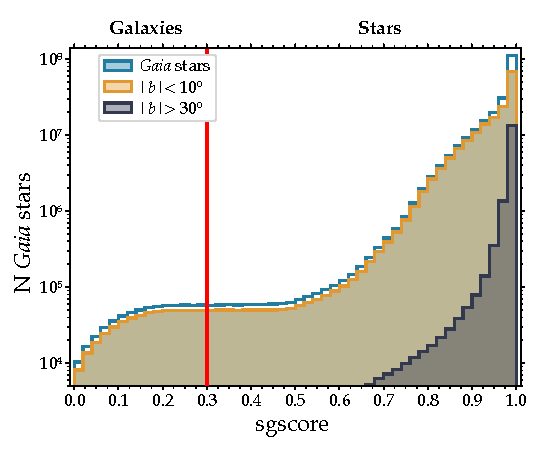
\includegraphics{nuclear/sgscore.pdf}
  \caption[\texttt{sgscore} performance]{\texttt{sgscore} performance evaluated with known \textit{Gaia} stars. At the chosen threshold of 0.3 (red line), the misidentification of stars as galaxies is negligible. Adapted from~\cite{Tachibana2018}}
  \labfig{sgscore}
\end{marginfigure}

The criteria used in this study were as follows:
\begin{description}
  \item[\texttt{sgscore}] As detailed in Section~\ref{ztf_image_subtraction}, \texttt{sgscore} is a machine-learning based star-galaxy score for PS1 objects (low values: galaxy, high values: stars). The transient at least once needed to have an \texttt{sgscore} < 0.3 to pass the filter.
  \item[Number of detections] At least 3 detections in both ZTF \textit{g}- and \textit{r}-band were required.
  \item[Proximity to galactic plane] The object had to be separated by at least \SI{5}{\degree} from the galactic plane to avoid contamination by foreground stars.
  \item[PS1 photometry] To avoid crowded areas, transients for which more than 100 objects in the vicinity had a counterpart in PS1 were removed.
  \item[Brightness] At least one alert datapoint of the transient had to be brighter than 20 mag.
  \item[\texttt{rbscore}] The real-bogus score separating erroneous detections (low values) from real ones (high values, see Section~\ref{ztf_alerts}) must be larger than 0.3. Note that for more recent data, also \texttt{deep real bogus} is available, which promises considerably better results~\sidecite{Duev2019}. Unfortunately, alerts from 2018 or 2019 do not contain this information, and there is no direct translation from an \texttt{rbscore} threshold to a \texttt{drbscore} threshold or re-analysis of the older alerts available. For these reasons and to maximize consistency, I restricted myself to using only the older \texttt{rbscore}. The quite loose cut of 0.3 does not entail overly large contamination, as I also required the transient to have a PS1 counterpart. Figure~\ref{fig:rbvsdrb} shows a comparison of the False Negative Rate (FNR) of \texttt{rbscore} vs. \texttt{drbscore}. At the chosen threshold of $0.3$, the FNR for both algorithms lies at the percent level.
  \item[Core distance] For all objects that made it this far, their angular distance to the core was computed. To make this more robust, three different distance metrics were employed: The mean distance to the PS1 source in the reference images, the median distance to that, and lastly, a weighted distance. The latter was computed according to~\sidecite{Velzen2019} and accounts for the fact that the RMS of the angular core distance scales linearly with magnitude. $\sigma_\text{dist}$ = $0.24 + 0.04(m-20)$, where $m$ is the difference photometry magnitude. This stage accepted all transients for which at least one of the three angular distances lay below \SI{0.5}{\arcsec}.
\end{description}

\begin{figure}[htpb]
  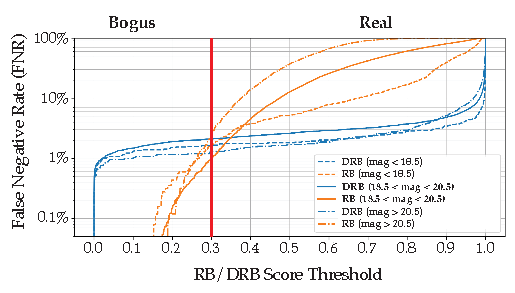
\includegraphics[width=0.9\textwidth]{nuclear/rb_v_drb.pdf}
  \caption[\texttt{rbscore}/\texttt{drbscore} performance]{\texttt{rbscore} vs \texttt{drbscore} performance, evaluated in terms of false negative rate as a function of the threshold. Adapted from~\cite{Duev2019}. The chosen threshold of 0.3 is shown as red vertical line. At that value, \texttt{rbscore} has a False Negative Rate of \SI{\approx1}{\percent} in the relevant magnitude range of $18.5 < \text{mag} < 20.5$.}
  \labfig{rbvsdrb}
\end{figure}

This filter was applied to all ZTF alerts issued between 1 April, 2018 and 30 April, 2022, comprising over 4 years of data in total.

\subsection{Rejection Statistics}
From a total sample of $\sim 350$ Million alerts issued by ZTF during these 4 years, ultimately 11,687 nuclear transients were selected. The survival rates during the filtering process are shown in Fig.~\ref{fig:nuclear_decision}, with the complete alert stream on top, different thematically grouped rejection stages in between and the final accepted alerts on the bottom. In total, \SI{0.2}{\percent} of alerts issued by ZTF were accepted by the filter.

\begin{figure}[h!]
  \begin{tikzpicture}[node distance=1.4cm]
    \node (start) [keep] {355,429,833 initial ZTF alerts};
    \node (dec1) [decision,  font=\small, align=center, below of=start] {SQL Filter};
    \node (expl1) [explain, font=\small, align=left, left of=dec1, xshift=-1.8cm] {$<20$ mag\\\texttt{rbscore} $>0.3$\\PS1 dist $<0.5$ arcsec\\$\geq 3$ detections};
    \node (disc1) [discard, font=\small, right of=dec1, xshift=2.48cm] {Discard alerts};
    \node (dec1a) [decision, font=\small, align=center, below of=dec1] {Transient\\already accepted?};
    \node (keep1) [keep, font=\small, below of=dec1a] {Retain 81,387,053 alerts};
    \node (dec2) [decision, font=\small, align=center, below of=keep1] {\texttt{sgscore}\\veto};
    \node (expl2) [explain, font=\small, align=left, left of=dec2, xshift=-2.2cm] {\texttt{sgscore} $\leq0.3$};
    \node (disc2) [discard, font=\small, right of=dec2, xshift=2.44cm,align=center] {Discard\\81,204,804\\alerts};
    \node (keep2) [keep, font=\small, below of=dec2] {Retain 182,080 alerts};
    \node (dec3) [decision, font=\small, align=center, below of=keep2] {PS1\\veto};
    \node (expl3) [explain, font=\small, align=left, left of=dec3, xshift=-1.5cm] {PS1 source faint enough\\good PS1 photometry};
    \node (disc3) [discard, font=\small, right of=dec3, xshift=2.5cm, align=center] {Discard\\20,331 alerts};
    \node (keep3) [keep, font=\small, below of=dec3] {Retain 161,749 alerts};
    \node (dec4) [decision, font=\small, align=center, below of=keep3] {Photometry\\veto};
    \node (expl4) [explain, font=\small, align=left, left of=dec4, xshift=-1.5cm] {$<20$ mag\\$\geq$ 3 detections\\flux increase $>2.5$ mag};
    \node (disc4) [discard, font=\small, right of=dec4, xshift=2.5cm, align=center] {Discard\\68,985 alerts};
    \node (keep4) [keep, font=\small, below of=dec4] {Retain 92,764 alerts};
    \node (dec5) [decision, font=\small, align=center, below of=keep4] {Position\\veto};
    \node (expl5) [explain, font=\small, align=left, left of=dec5, xshift=-1.5cm] {$>5$ deg from gal. plane\\not potential mover};
    \node (disc5) [discard, font=\small, right of=dec5, xshift=2.5cm, align=center] {Discard\\38,600 alerts};
    \node (keep5) [keep, font=\small, below of=dec5] {Retain 54,164 alerts};
    \node (dec6) [decision, font=\small, align=center, below of=keep5] {\textit{Gaia}\\veto};
    \node (expl6) [explain, font=\small, align=left, left of=dec6, xshift=-1.5cm] {No match to \textit{Gaia} star\\$\leq30$ \textit{Gaia} stars close by};
    \node (disc6) [discard, font=\small, right of=dec6, xshift=2.5cm, align=center] {Discard\\42,477 alerts};
    \node (keep6) [keep, font=\small, below of=dec6] {Keep 723,053 alerts};
    \node (keep7) [keepfinal, font=\small, below of=keep6] {Keep 11,687 transients};
    \draw [arrow] (start) -- (dec1);
    \draw [arrow] (keep1) -- (dec2);
    \draw [arrow] (dec1) -- node[midway,above] {\small no} (disc1);
    \draw [arrow] (dec1) -- node[midway,left] {\small yes} (dec1a);
    \draw [arrow] (dec2) -- node[midway,above] {\small no} (disc2);
    \draw [arrow] (dec2) -- node[midway,left] {\small yes} (keep2);
    \draw [arrow] (dec1a) -- node[midway,left] {\small no} (keep1);
    \draw [arrow] (keep2) -- (dec3);
    \draw [arrow] (dec3) -- node[midway,above] {\small no} (disc3);
    \draw [arrow] (dec3) -- node[midway,left] {\small yes} (keep3);
    \draw [arrow] (keep3) -- (dec4);
    \draw [arrow] (dec4) -- node[midway,above] {\small no} (disc4);
    \draw [arrow] (dec4) -- node[midway,left] {\small yes} (keep4);
    \draw [arrow] (keep4) -- (dec5);
    \draw [arrow] (dec5) -- node[midway,above] {\small no} (disc5);
    \draw [arrow] (dec5) -- node[midway,left] {\small yes} (keep5);
    \draw [arrow] (keep5) -- (dec6);
    \draw [arrow] (dec6) -- node[midway,above] {\small no} (disc6);
    \draw [arrow] (dec6) -- node[left] {\small yes} (keep6);
    \draw [arrow] (dec1a.east) -- ++(4,0) node[midway,above]{\small yes} |- (keep6.east);
    \draw [arrow] (keep6) -- node[midway,left] {\small translates to} (keep7);
  \end{tikzpicture}
  \caption[Nuclear filter flow chart]{Flow chart showing the rejection statistics of the nuclear filter.}
  \labfig{nuclear_decision}
\end{figure}

As one can see, the vast majority of alerts were rejected based on them being either too faint, likely being bogus, or likely being stars. The majority of alerts already got filtered out by the initial SQL query. The SQL-based filtering was also the most efficient one, so I ensured that the amount of filtering at that stage (on the archive server) was maximized.

This was followed by the live transfer of all surviving alerts to another machine and processing of the subsequent filtering stages. In total, the filtering process took roughly 5 weeks.

\subsection{Forced photometry}
To be sensitive to early and late-time light curve evolution, forced photometry was acquired for all 11,687 transients making the final cut. This was again done with \texttt{fpbot}, see Section~\ref{fpbot} for details. The process proved somewhat cumbersome due to the enormous data volume (several hundreds of GB) that was required to be transferred from IPAC and stored and processed in batches due to computing center restrictions.

\subsection{Infrared Data}\label{irdata}
Motivated by the strong dust echo detected for \textit{AT2019dsg}, \textit{AT2019fdr} and \textit{AT2019aalc}, the optical forced photometry dataset was complemented with infrared light curves from the \textit{WISE} mission. These were obtained to serve in a selection of interesting transients based on their infrared dust echo, see Section~\ref{dustecho_sel}.

Data retrieval was performed with the \texttt{timewise} package~\sidecite{Necker2023a} to download all datapoints available for each source location in the \textit{W1}- and \textit{W2}-band. The tool automatically crossmatched the ZTF transient position to the \textit{WISE} light curve repository, downloaded the photometry for each source and binned the single source exposures of each epoch, spaced in half-year intervals.

Most sources did have infrared counterparts. To obtain a selection of likely dust-echo candidates, two \texttt{AMPEL} packages (\texttt{T2BayesianBlocks} and \texttt{T2DustEchoEval}) were used to analyze the infrared light curves with a Bayesian block algorithm in order to identify periods of flaring activity compared to a baseline; see also Section~\ref{bayesian_blocks} for a discussion of the same algorithm utilized for ZTF optical data.

The significance of these flares was then calculated with a metric dubbed `dust echo strength'. This was defined in~\cite{Velzen2021} as $\Delta F_\text{IR}/F_\text{RMS}$, where $\Delta F_\text{IR}$ is the difference between the flaring period flux and the baseline flux, while $F_\text{RMS}$ is the root mean square of the baseline flux.

\subsection{Catalog Matching}
To enrich the sample by information available on the transients, these were crossmatched to a variety of catalogs and services. The results of the crossmatches were stored locally in a \texttt{MongoDB} database for ease of retrieval. The crossmatches were either used to extract training features (e.g.~\textit{WISE} colors) or evaluate the quality of the trained models (e.g.~GROWTH Marshal, Fritz or TNS). In detail, these crossmatches comprised:

\begin{description}
  \item[Spectroscopic Redshifts] To obtain spectroscopic redshifts, the \texttt{AMPEL} module \texttt{T2DigestRedshifts} was employed. This queries the following services: A local database of the spectroscopic redshifts contained in the NASA/IPAC Extragalactic Database (NED)\sidenote{\url{https://ned.ipac.caltech.edu}}, spectroscopic redshifts from SDSS, and finally spectroscopic redshifts from the Galaxy List for the Advanced Detector Era (GLADE)~\sidecite{Dalya2018} v2.3.
  \item[Photometric Redshifts] Additionally, \texttt{T2DigestRedshifts} also provided photometric redshifts from the Legacy Survey~\sidecite{Zhou2020}, the 2MASS Photometric Redshift Catalog~\sidecite{Bilicki2013}, and photometric redshifts from the PS1 Source Types and Redshifts with Machine learning (PS1-STRM) catalog~\sidecite{Beck2020} as well as GLADE.
  \item[GROWTH Marshal/Fritz] During ZTF Phase I, the GROWTH Marshal~\sidecite{Kasliwal2019} served as a community hub to gather information on single transients. It provided a web interface to upload spectroscopy, discuss photometry and add classifications and redshift. This service has been replaced by Fritz~\sidecite{Coughlin2023} with the same design goal, but greater modularity and API support. Both services were queried for transient classifications and redshifts.
  \item[TNS] The Transient Name Server (see Section~\ref{catmatch}) was also used to obtain classifications and redshifts of known transients.
  \item[AllWISE] Additionally to the \textit{WISE} light curves, archival data from the first part of the \textit{WISE} mission was obtained. This dataset had the advantage of providing two additional bands reaching into the far infrared (\textit{W3} and \textit{W4}), both of which were deactivated after the nominal mission end of \textit{WISE} due to lack of coolant. These allowed for the calculation of more colors, which were used in AGN rejection, see Section~\ref{agn_rejection}.
  \item[CRTS DR1] The Catalina Real-time Transient Survey Catalog contains cataclysmic variables which were crossmatched against to reduce contamination by foreground stars.
  \item[SDSS] The Sloan Digital Sky Survey was also used to crossmatch against foreground stars.
\end{description}

\section{Creating Features: Light Curve Fits}
To photometrically classify the transients, the following strategy was employed: Fit all transients with a dedicated TDE light curve model, as well as a supernova Ia model. The features extracted from these fits, appended by additional ones, served as a base to classify the nuclear sample. Such a training task required a truth on which to train on. The truth base chosen here was the BTS sample, which was augmented by creating copies of existing objects, as well as adding new, underrepresented transients. All those steps will be explained below.

\subsection{Fitting a TDE Model}\label{tde_model}
To model a TDE-like source evolution, a variation of the parametrization presented in~\cite{Velzen2021a} was used.

\subsubsection{TDE Parametrization}
The basic  idea is to fit the light curve evolution with a Gaussian rise and exponential decay of a blackbody, which is also allowed to linearly change its temperature for a number of days. The luminosity evolution is then given by

\begin{equation}
  L(t,\lambda) = \frac{T_\text{peak}^4}{T(t)^4} B_\lambda F(t),
\end{equation}
where $\lambda$ is the evaluated wavelength, $T_\text{peak}$ is the blackbody temperature at peak, $T(t)$ is its temperature at time $t$ and $B(t)_\lambda$ is the spectral radiance of the blackbody. $B(t)_\lambda$ is given by
\begin{equation}
  B(t)_\lambda = \frac{2 c h}{\lambda^5} \frac{1}{\exp(\frac{hc}{\lambda k_B T(t)})-1},
\end{equation}
and $F(t)$ is the Gaussian rise pre-peak and exponential decay post peak, given by
\begin{equation}
  F(t) = \begin{cases}
    \exp[-(t-t_\text{peak})^2/2\sigma^2] & \text{if } t\leq t_\text{peak} \\
    \exp[-(t-t_\text{peak})/\tau]        & \text{otherwise.}
  \end{cases}
\end{equation}
Here, $\sigma$ is the rise time of the transient, and $\tau$ is the decay time, both in days.

Lastly, $T(t)$ was allowed to change linearly during an interval after $t_\text{peak}$ until $t_\text{cutoff}$, marking the end of the linear temperature evolution:
\begin{equation}
  T(t) = \begin{cases}
    T_\text{peak}                    & \text{if $t<t_\text{peak}$}                              \\
    T_\text{peak} + t \cdot \Delta T & \text{if $~t_\text{peak} \leq t \leq t_\text{cutoff} $ } \\
    T_\text{cutoff}                  & \text{otherwise},
  \end{cases}
\end{equation}
with $\Delta T$ being the coefficient of temperature change. Also, there was a check that required at least 10 datapoints within the time interval 30 days prior to peak time and one year after that. If that check did not succeed, the fit was set to fail due to poor source sampling.

As a source luminosity can only be calculated when the redshift is known, and this was not the case for a majority of the nuclear transients, an arbitrary amplitude was used instead. This does not affect the results in any meaningful way, as TDEs can differ in brightness by at least two orders of magnitude (see e.g.~\cite{Hammerstein2022}), and only the shape of the light curve is relevant for the goodness of fit\cite{Hammerstein2022}.

This model has been realized as an instantiation of an \texttt{SNCosmo} source model, as this package had the advantage of built-in filter profiles which allowed the correct evaluation of the blackbody flux as seen through the ZTF bandpass filters. To make the fit procedure computationally feasible, the algorithm used was not a Markov-Chain Monte Carlo as in~\cite{Velzen2021a}, but \texttt{iminuit/MIGRAD}.

To account for Milky Way dust extinction along the line of sight, the infrared dust maps by Schlegel, Finkbeiner \& Davis were used~\sidecite{Schlegel1998}, as provided by the \texttt{sfdmap}\sidenote{\url{https://github.com/kbarbary/sfdmap}} Python package.

\subsubsection{TDE Fit Priors}
To constrain the fits and mitigate runaway, fit priors were used, partly taken from~\cite{Velzen2021a}. These are shown in Table~\ref{tab:tde_fit_priors}.

The prior on the time of peak, here dubbed $t_0$, was inferred from a peak-finding algorithm that identified the highest flux point in each band (given it had a signal-to-noise ratio of $>3$) after smoothing the light curve with a rolling window, calculating the median flux within a window of 10 days.

\begin{table}[h]
  \begin{center}
    \begin{tabular}{c c c c}
      \hline
      \textbf{Param.}      & \textbf{Description} & \textbf{Prior} & \textbf{Bounds}                     \\
      \hline
      \hline
      $t_\text{peak}$      & Peak time            & $t_0$          & $t­_0 \pm 30$ days                  \\
      $\log T_\text{peak}$ & Peak temperature     & 4 K            & [3.5, 5]~\unit{\K}                  \\
      $\log \sigma$        & Gaussian rise time   & 1.6 days       & [0,5] days                          \\
      $\log \tau$          & Exp. decay time      & 2.3 days       & [0,5] days                          \\
      $\Delta T$           & Temp. change / day   & 0              & $T_\text{peak} \pm 15000$ K (total) \\
      $t_\text{cutoff}$    & End of temp. evol.   & 300            & [100, 1200] days $+t_0$             \\
      \hline
    \end{tabular}
  \end{center}
  \caption[TDE Fit priors]{Priors for the TDE fit.}\label{tab:tde_fit_priors}
\end{table}

As the blackbody fits were not constrained by UV data, in some cases a temperature runaway occurred when allowing all fit parameters to vary freely within their bounds. This can be explained as follows: A decrease in brightness over time can either be achieved by exponential decay or by an increase in temperature. The latter gradually moves the blackbody spectrum outside the ZTF bands, which then translates to a decrease in brightness. As such excessive temperature changes are most likely unphysical, the daily temperature change $\Delta T$ was limited to an integrated maximum change of $T_\text{peak} \pm \SI{1.5e4}{\K}$.

Another measure to mitigate the issue was to perform the fits as a two-stage process: First, the temperature evolution was neglected, i.e. $\Delta T$ was set to $0$ and $t_\text{cutoff}$ was removed as parameter, with the blackbody only having one temperature for the duration of the light curve, $T_\text{peak}$. The best-fit values for $t_\text{peak}$, $\log T_\text{peak}$, $\log \sigma$ and $\log \tau$ obtained in this first stage were then used as fit priors for stage 2. This procedure solved the temperature runaway in almost all cases.

\begin{figure}[htb]
  \centering
  \begin{subfigure}[b]{0.49\textwidth}
    \centering
    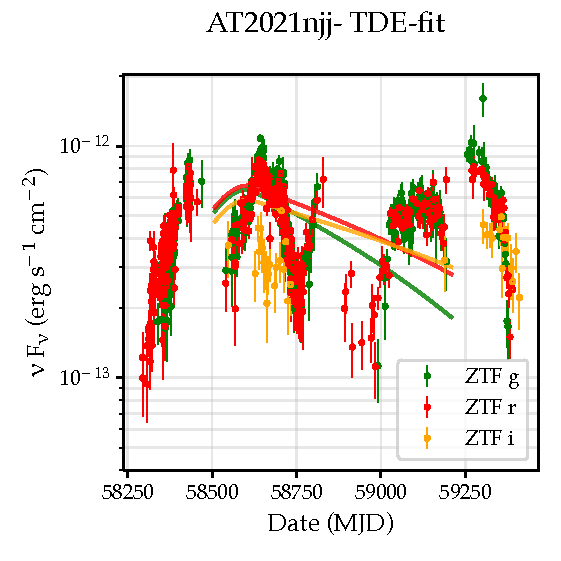
\includegraphics[width=1\textwidth]{nuclear/ZTF18aaymybb_exp.pdf}
  \end{subfigure}
  \begin{subfigure}[b]{0.49\textwidth}
    \centering
    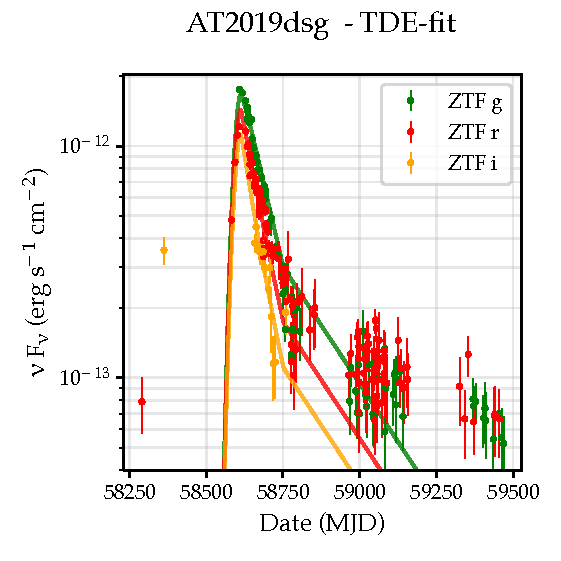
\includegraphics[width=1\textwidth]{nuclear/ZTF19aapreis_exp.pdf}
  \end{subfigure}
  \caption[Two exemplary TDE fits]{Two exemplary TDE light curve fits. Left: \textit{AT2021njj}, displaying periodic AGN activity not well captured by the fit.\ Right: \textit{AT2019dsg}, a TDE which is captured fairly well by the fit routine.}
  \labfig{tde_fit_comparison}
\end{figure}

Fig.~\ref{fig:tde_fit_comparison} shows two exemplary TDE fits; one for an object of unknown nature (\textit{AT2021njj}) on the left and one for a confirmed TDE (\textit{AT2019dsg}, see Section~\ref{at2019dsg}) on the right. As one can see, the fit captures the light curve evolution of the TDE fairly well, including the change in color due to the changing blackbody temperature.~\textit{AT2021njj} on the other hand---whatever it actually is (the object has no spectroscopic classification)---is clearly not a TDE. The fit cannot account for the periodic nature of the object, resulting in a reduced $\chi^2$ of $26.3$.

The successful fit for \textit{AT2019dsg} meanwhile results in the following values: A reduced $\chi^2$of $4.1$, a peak temperature of \SI{8700}{\K} which decays by \SI{78}{\K} per day for the following 138 days, an initial risetime of 21 days, and a characteristic light curve decay time of 216 days.

This object nevertheless highlights a restriction: The available optical to infrared data from ZTF does not constrain blackbodies well. When including additional UV data for \textit{AT2019dsg} near light curve maximum, the inferred blackbody temperature is \SI{4e4}{\K}, significantly higher. This is not a failure of the fit procedure, but driven by the high UV flux pushing the blackbody to shorter wavelengths (the additional UV data can be seen in Fig.~\ref{fig:at2019dsg_lc}).

\subsection{Fitting a SN Ia Model}\label{salt}
As SNe Ia are a prominent contaminant for bona fide nuclear events (i.e.~such events that can only occur in the centers of galaxies), it was crucial to identify them. To achieve this goal, all light curves were additionally subjected to a fit using the tried and tested Spectral Adaptive Lightcurve Template (SALT2)~\sidecite{Guy2007} SN Ia light curve model.

SALT2 assumes that the light curve is indeed a supernova Ia and applies empirical corrections to the light curve color and stretch (i.e.~the width of the light curve). This is achieved by matching templates generated by a set of well-sampled Ia light curves and spectra of varying distance. The resulting color and stretch correction parameters, as well as the peak brightness and the reduced $\chi^2$ were saved and will later be used as features in training the classifier.

\begin{figure}[H]
  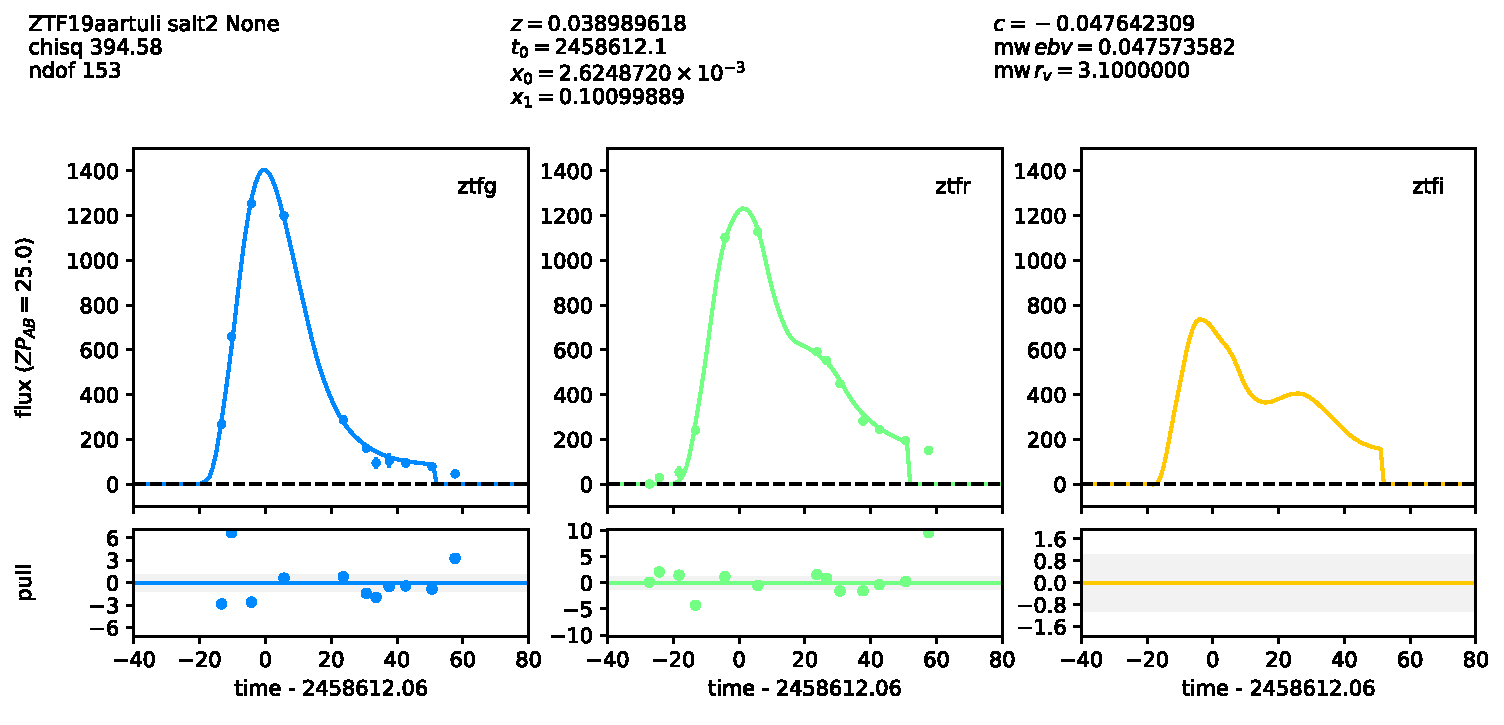
\includegraphics[width=1\textwidth]{nuclear/salt.pdf}
  \caption[SALT2 Fit]{Exemplary SALT2 fit output. The three panels show three ZTF bands of \textit{AT2019dzzo}, a spectroscopically confirmed SN Ia. Time 0 is the fitted peak of the assumed SN Ia; and as one can see the transient in question is fairly well approximated by SN Ia light curve, with a reduced  $\chi^2=2.67$.}
  \labfig{salt2}
\end{figure}

The fits were performed with \texttt{SNCosmo}, which itself fits the light curves using \texttt{iminuit/MIGRAD}.

\section{Creating Features: Optical Flare Analysis}\label{bayesian_blocks}
Another feature which will later be used in the classification of transients were simultaneous flares across the well-sampled ZTF \textit{g}- and \textit{r}-bands. The number and timing of optical flares within different bands can then be used to differentiate between different types of transients.

\subsection{Bayesian Block Algorithm}\label{bayesian_block}
To determine time periods of heightened activity, a Bayesian block algorithm was employed. This was a version of a package developed at DESY, modified by the author to analyze optical ZTF light curves instead of infrared \textit{WISE} data.

The Bayesian block algorithm is explained in~\sidecite{Scargle1998,Scargle2013}; the implementation used here is integrated in the \texttt{astropy} package. The light curves were first smoothed by calculating the median and standard deviation within a 10-day rolling window. After that, only data points lying within $3 \sigma$ distance in magnitude space from the median were used. This got rid of flux outliers, which were quite frequent for the forced photometry light curves of the nuclear sample.

The Bayesian block algorithm uses a prior on the number of blocks $N_\text{blocks}$, which is computed as $P(N_\text{blocks})= P_0 \gamma^{N_\text{blocks}} $, where $P_0$ is a normalization dependent on the number of datapoints $N$. For this analysis, the prior was computed with a slope $\gamma$ of $\gamma = N ^{-10/\ln{10}} $, with $N$ being the number of datapoints in the smoothed single-band light curve. The slope $\gamma$ was determined empirically to yield robust results. It was a compromise between sensitivity to flux changes and detecting too many blocks, each too small to be meaningful.

\subsection{Block Coincidence}
As they were much better sampled than the \textit{i}-band, the \textit{g}- and \textit{r}-band were used to check for blocks temporally coincident in both bands.

For this, each region with increased flux compared to a baseline in the \textit{g}-band was checked to see if there was a corresponding \textit{r}-band block with increased flux overlapping in time.

\begin{figure}
  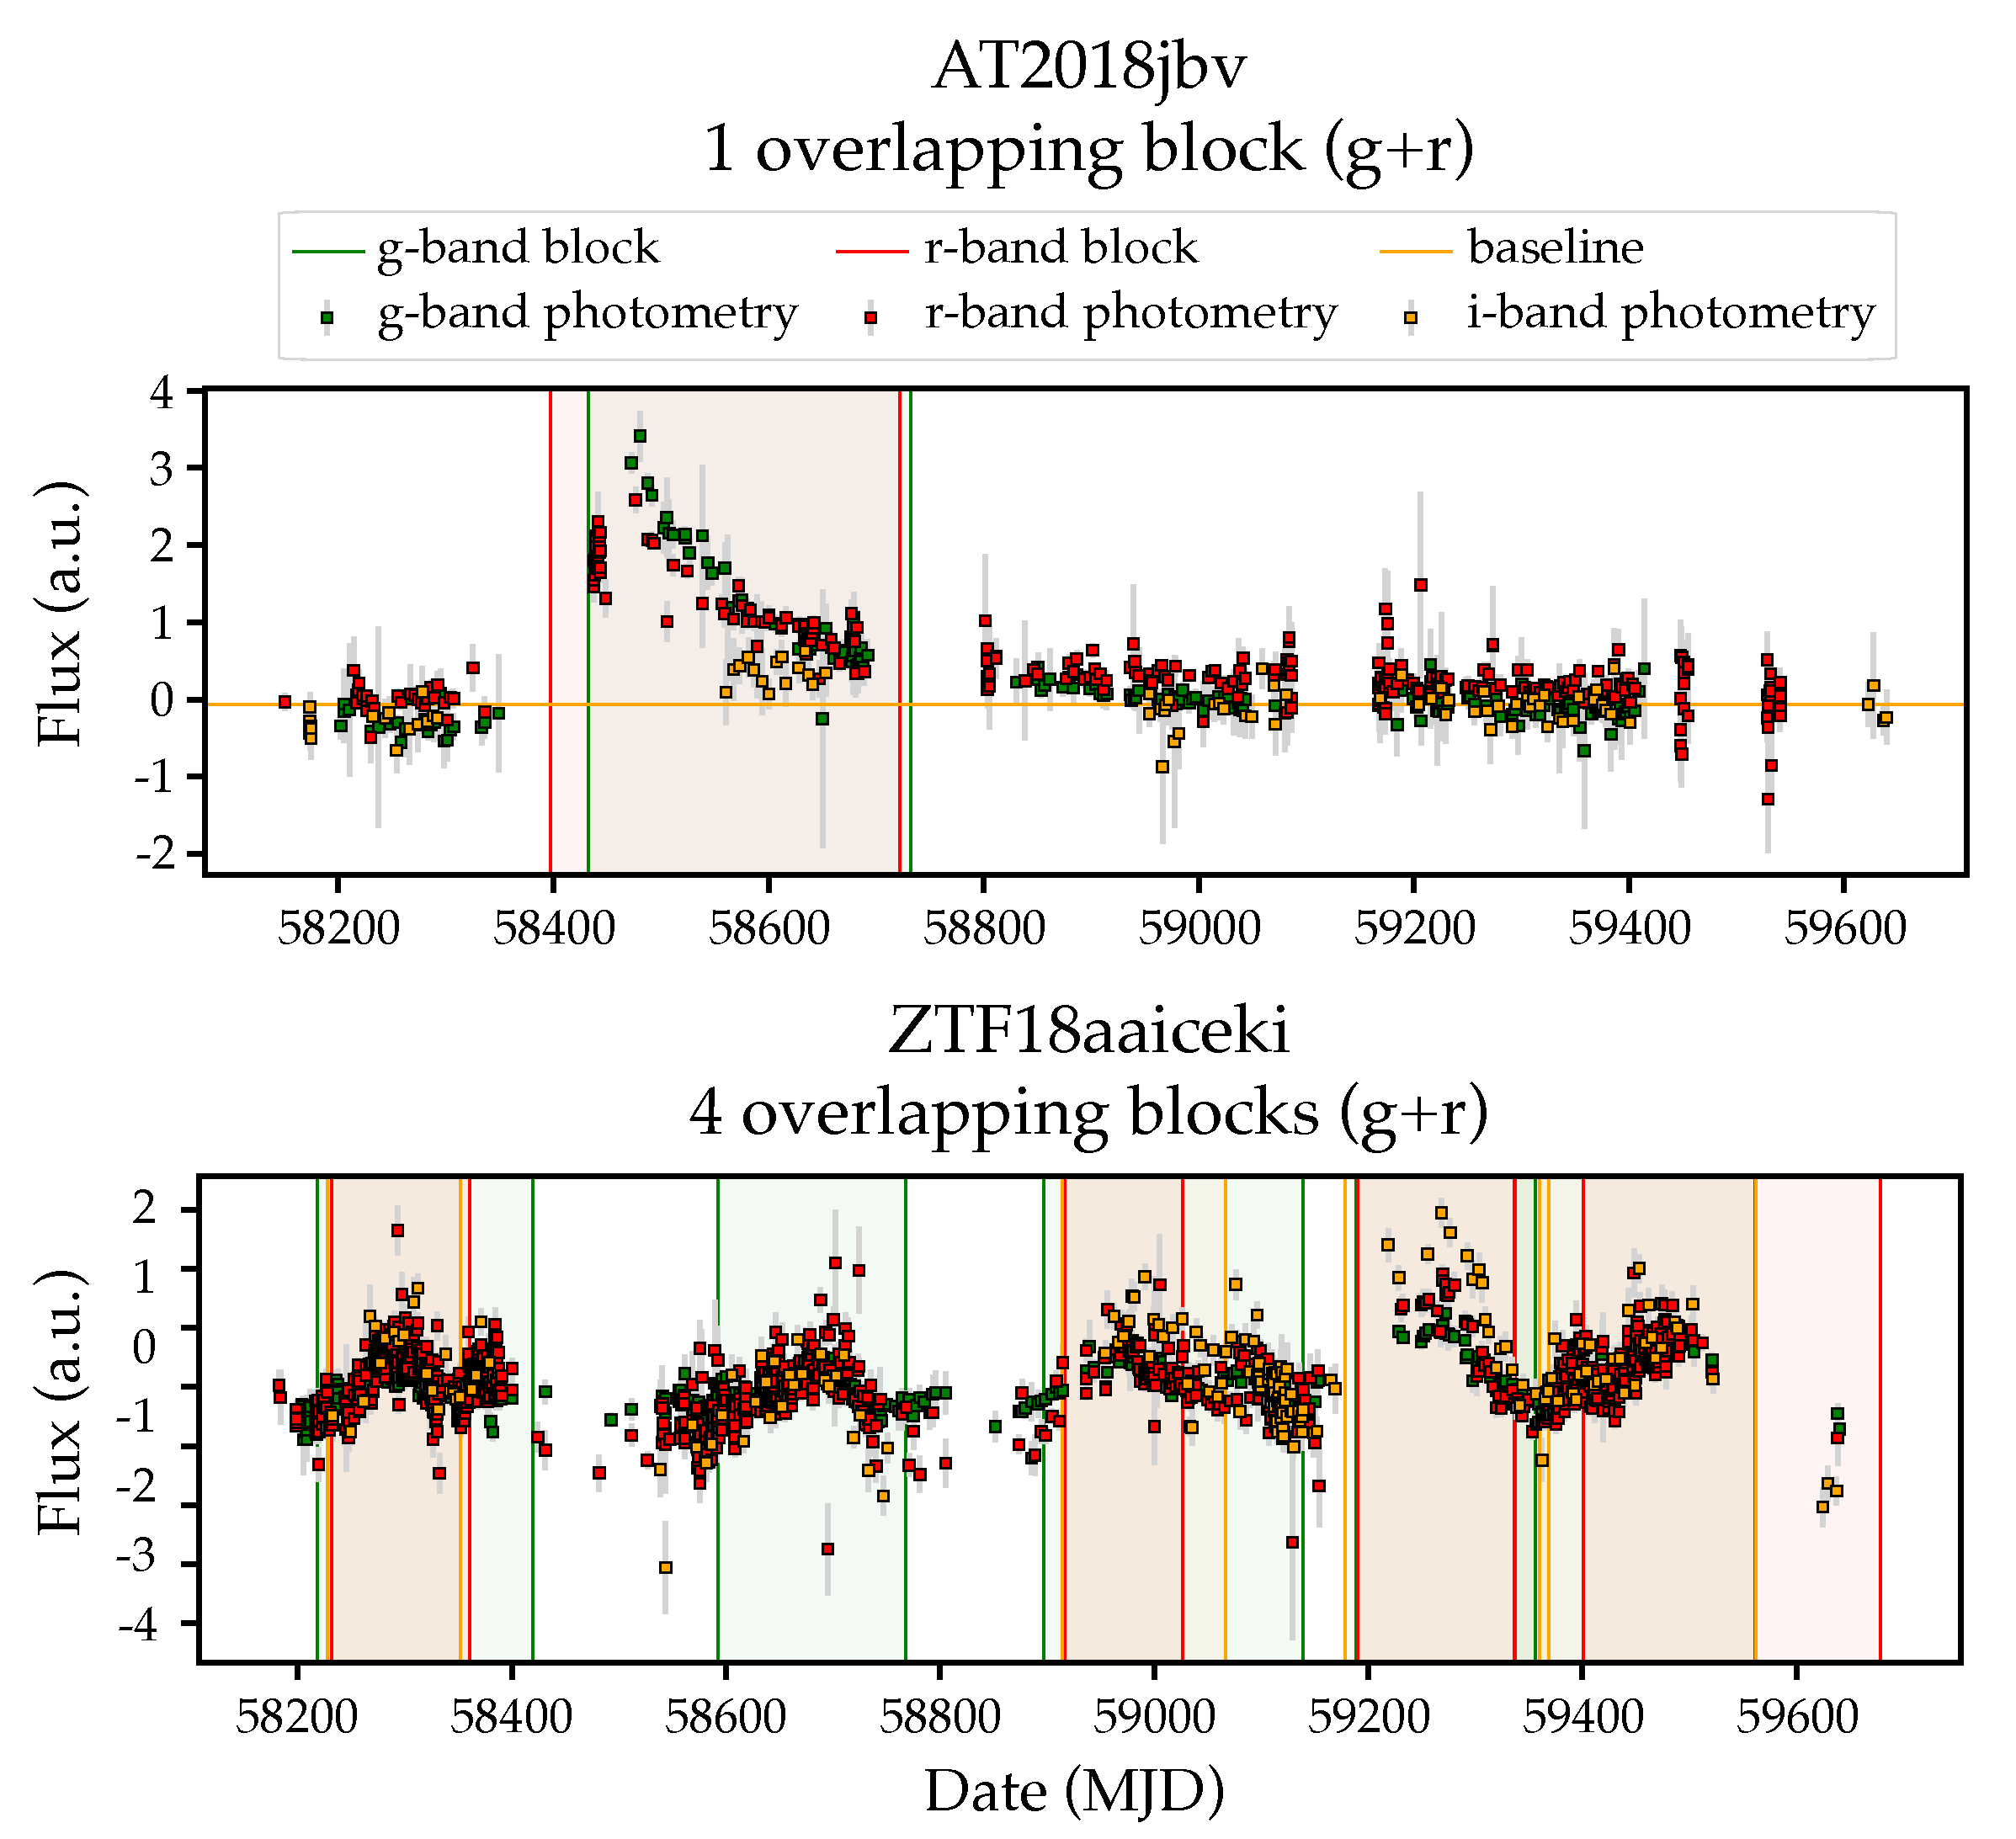
\includegraphics[width=1\textwidth]{nuclear/bayesian_blocks.pdf}
  \caption[Bayesian blocks]{Top: Bayesian Blocks identified for \textit{AT2018jbv}. There is one block both in \textit{g}- and \textit{r}-band, which overlaps. This is a strong indicator that the transient is a one-time flare, stemming from e.g.~a supernova or a TDE (the transient is in fact a TDE), in contrast to stochastic AGN variability. Bottom: Bayesian Blocks for \textit{ZTF18aaiceki}, showing AGN activity. This is correctly captured by a large number of overlapping regions.}
  \labfig{bayesian_blocks}
\end{figure}

One can see two examples of such overlapping blocks in Fig.~\ref{fig:bayesian_blocks}, which shows the result of the Bayesian Block algorithm for \textit{AT2018jbv} and \textit{ZTF18aaiceki}. Both are transients from the nuclear sample, the first one being a TDE, the second an AGN displaying stochastic variability.

\section{Training Sample}
As one of the goals was the classification of the nuclear sample, a training sample that most closely resembled the target sample in brightness needed to be chosen.

\begin{marginfigure}
  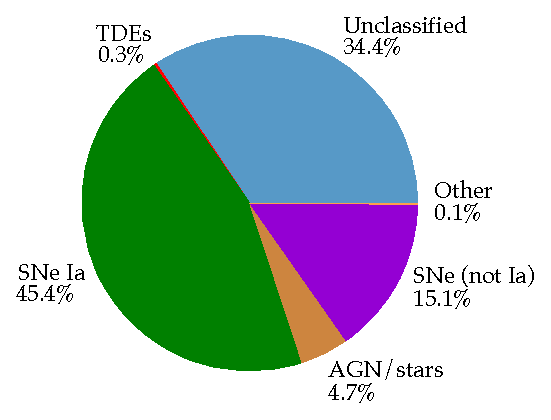
\includegraphics{nuclear/BTS_full.pdf}
  \caption[BTS Composition]{Composition of the Bright Transient Survey sample used in this study. The classified part of the sample is heavily biased towards SNe Ia, AGN are vastly under-sampled.}
  \labfig{bts_composition}
\end{marginfigure}

\subsection{The Bright Transient Survey}\label{bts}
The natural starting point for the creation of a training sample was the so-called ZTF Bright Transient Survey (BTS)\sidenote{\url{https://sites.astro.caltech.edu/ztf/bts/bts.php}}, see~\cite{Fremling2020,Perley2020} for details. The basic goal of the survey was the spectroscopic classification of all ZTF-detected transients brighter than 18.5 mag in either the \textit{g}- or \textit{r}-band. It even managed to push further, achieving a spectroscopic completeness of \SI{75}{\percent} at 19 mag (\SI{93}{\percent} at the nominal cutoff of 18.5 mag)~\cite{Perley2020}.

This was achieved by utilizing the fully robotic SED machine for quick classification, and employing other spectroscopic resources for ambiguous spectra. BTS is the largest spectroscopic supernova survey ever conducted, with over 8000 classified transients as of August 2023.

There were three potential issues that needed to addressed though when using the BTS as starting point for a training sample:

\begin{description}
  \item[Brightness bias] The BTS restriction to objects usually brighter than 18.5 mag means that the majority of the BTS sample is brighter than the nuclear sample with its magnitude cut of 20.
  \item[Class imbalance] The BTS is heavily skewed towards supernovae. Also, because SNe Ia are brighter, the majority of the SNe contained in a flux-limited sample like the BTS are of type Ia~\cite{Perley2020}, with \SI{70}{\percent} of all classified BTS transients being SNe Ia. This results in a class imbalance of the training sample.
  \item[Anti-AGN bias] To reduce contamination stemming from AGN variability, the BTS vetoes transient host galaxies that likely harbor an AGN. This is achieved by crossmatching candidate sources to known AGN, based on \textit{WISE} color cuts, or by rejecting sources with previous variability most likely hinting at AGN activity. This poses a problem: As the nuclear sample will contain a large number of AGN, this also results in a class imbalance.
\end{description}

These issues needed to be solved somehow. Two procedures to do that will be described below: Augmentation by creating fainter copies addressed the brightness bias and partially the class imbalance, while rejecting likely AGN within the nuclear sample and expanding the training set with known AGN were both employed to deal with the anti-AGN bias.

\subsection{Augmentation: Enhancing the Training Set}\label{noisification}
One promising strategy was to multiply the number of light curves available by simulating observations of the same object at higher redshifts.

The method of augmentation employed here was developed by A. Townsend and the author. The procedure was implemented as Python package~\sidecite{Reusch2023c} and worked as follows:

\subsubsection{Draw new redshift}
A transient light curve (from now on: parent light curve) was obtained, as was its redshift $z_\text{parent}$ (all classified BTS transients have a spectroscopic redshift). A new redshift $z_\text{child}$ was drawn for the child light curve (i.e. the noisified copy) from a cubic redshift distribution ranging from $z­_\text{parent}$ to $z_\text{parent}+0.1$.

\subsubsection{Scale and scatter the flux}
After this, the parent flux was redrawn from a normal distribution centered around each parent flux value, scaled by its error. This was done to account for the fact that flux measurements are expected to scatter around their true value with their error, thereby simulating a `new' measurement which is more noisy due to the increased distance. After this, the re-drawn flux measurements were rescaled with the new redshift $z_\text{child}$. The flux $F$ scales according to $D_L=\frac{L}{4 \pi F}$ i.e.~with the square of the luminosity distance (see Section~\ref{fitmodels}). Therefore, one can determine a flux scaling factor $a$ according to
\begin{equation}
  a = \frac{D_L(z_\text{parent})^2}{D_L(z_\text{child})^2}.
\end{equation}
With this scaling factor, the child light curve flux is simply $f_\text{child} = a f_\text{parent}$.

The flux error got scaled accordingly, but with two additional empirical constant coefficients $e_f$ and $e_b$ determined by fitting the flux error as a function of flux. This procedure showed that the error $F_\text{err}$ deviates from the expected $\sqrt{F}$ behavior, but can be well approximated by $F_\text{err} = \sqrt{F + e_f^2\times F + e_b^2}$. The error as a function of flux, as well as the different approximations are shown in Fig.~\ref{fig:ztf_error_dist}. The factors $e_f$ and $e_b$ were determined as $e_f = 0.54$ and $e_b = 5.37$.

\begin{marginfigure}
  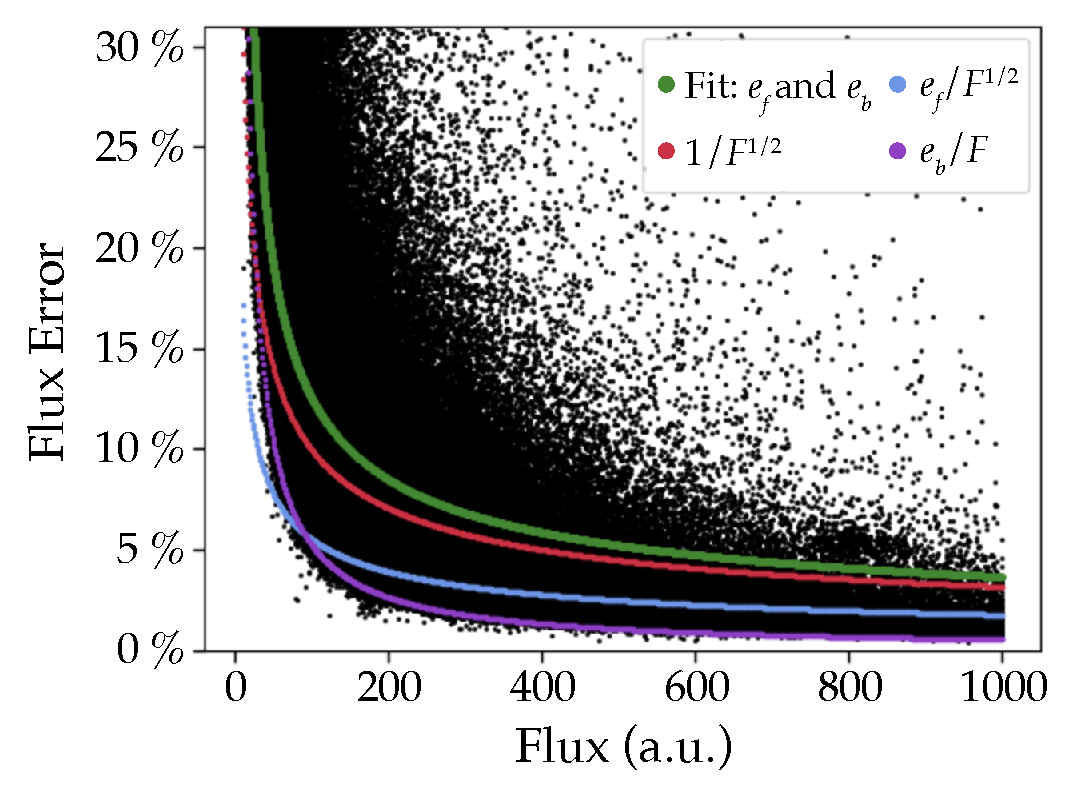
\includegraphics{nuclear/ztf_error_dist.pdf}
  \caption[ZTF error distribution]{ZTF error distribution: $F$ vs. $F_\text{err}$ in percentage of flux. The red curve shows the expected error behavior ($F_\text{err}\propto \sqrt{F})$, while the green curve shows the improved version $F_\text{err} = \sqrt{F + e_f^2\times F + e_b^2}$. Figure by A. Townsend with small modifications by the author.}
  \labfig{ztf_error_dist}
\end{marginfigure}

\subsubsection{Apply K-Correction}
If an \texttt{SNCosmo} model for the transient type existed, a K-correction was applied. This procedure accounts for the fact that by arbitrarily redshifting the light curve of an object, the spectrum will also be redshifted. Due to this, the ZTF bandpasses will register different parts of the spectrum, which leads to a different observed flux (see~\sidecite{Hogg2002} for an introduction).

\subsubsection{Scatter and sub-sample observations}
As a last step, the newly created light curve was sampled with a default retention fraction of 0.9, i.e.~\SI{10}{\percent} of datapoints were dropped randomly. Additionally, the observation times were slightly randomized to avoid creating regularities a machine-learning algorithm could pick up. This was achieved by scattering the observation dates around their original values, with a $\sigma$ of $0.03$ days.

\subsubsection{Reject faint light curves}
Finally, for each generated light curve, at least 5 datapoints were required to lie above a detection threshold of $5 \sigma$. If that requirement was not met, the light curve was discarded. This was implemented to mimic the nuclear filter (see Section~\ref{nuclear_filter}), which reacts to alerts issued by ZTF. Only datapoints with a signal-to-noise ratio of $>5$ warrant an alert, so the noisified light curves needed at least some datapoints above that threshold. The minimal number of detections for the noisified light curves was a bit higher compared to the nuclear filter (5 vs. 3) to account for the fact that forced photometry is slightly more sensitive than the PSF photometry used in the alerts.

\subsubsection{Sample dynamically}
Depending on the number of light curves for a specific class, the number of desired child light curves per parent light curve was determined to yield an augmented training set with balanced classes. For example, only 3 children per SN Ia light curve were generated, but up to 14 children per light curve of all other types of supernovae. The only exception were variable stars: For these, the redshift $\approx 0$ and could not be varied, so no children were generated.

The results of all these steps are exemplified in Fig.~\ref{fig:noisify_example}. It shows the light curve of an SN Ia, \textit{SN2019qym}, detected with a redshift of $z=0.02$. The original light curve can be seen, as well as a child light curve at higher redshift ($z=0.09$). Note the increased errors (the original object was very bright, so only one datapoint in the \textit{g}-band at 35 days after peak has visible error bars), the slightly different modified observation dates and the random removal of datapoints.

\begin{figure}[H]
  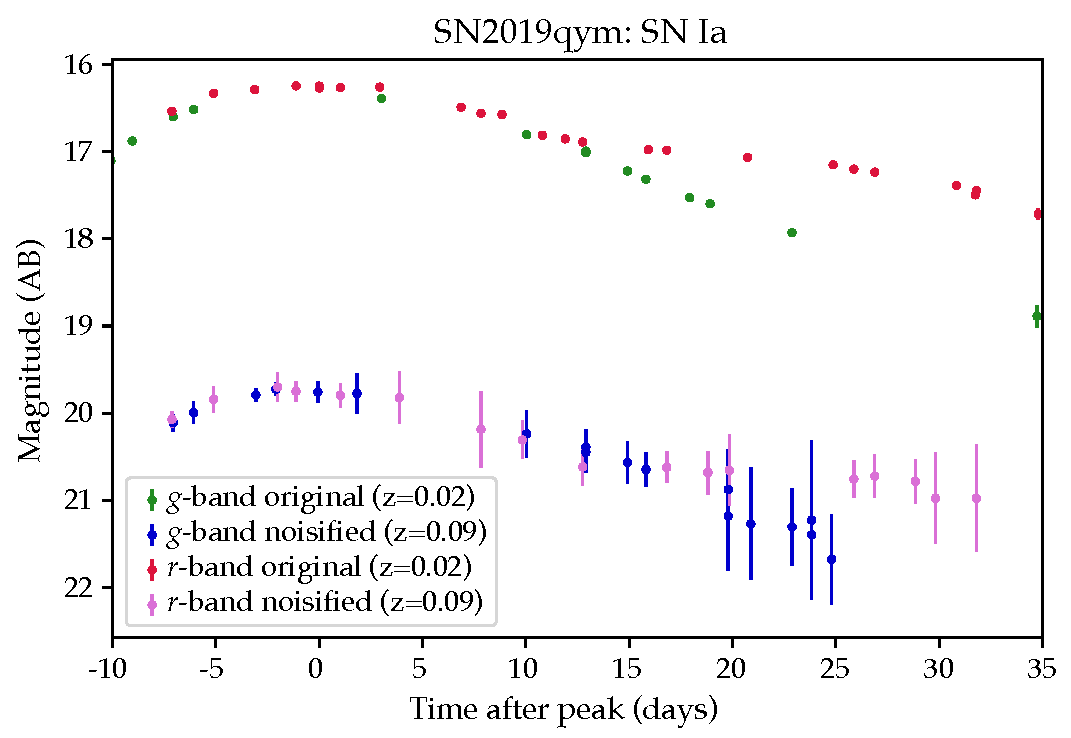
\includegraphics[width=1\textwidth]{nuclear/noisify_ZTF19acapeun.pdf}
  \caption[Augmentation example]{Original and `child' light curve of \textit{SN2019qym}, an SN Ia with a redshift of $z=0.02$. The original two bands are shown in green and red, while the fainter, noisier copy at a redshift of $z=0.09$ is displayed in blue and pink. Figure by A. Townsend, with slight modifications by the author.}
  \labfig{noisify_example}
\end{figure}

To match the anti-AGN bias within the BTS sample, in principle two methods are viable: Increase the number of AGN in the training sample, or veto against AGN in the sample that needs classification. To maximize performance, a combination of both approaches was chosen here, and each will be detailed in the next paragraphs.

\subsection{AGN Rejection}\label{agn_rejection}
Only those nuclear transients that survived the AGN rejection were kept for classification. The AGN rejection was performed as a two-step process, based on \textit{WISE}-colors and matches to the MILLIQUAS catalog.

\subsubsection{\textit{WISE} color selection}\label{wise_color_cut}
The cuts applied were taken from~\cite{Hviding2022}. The authors of that study evaluated roughly half a million SDSS galaxies with matching \textit{WISE} infrared data, resulting in a region within the \textit{WISE} color--color diagram that robustly picks out AGN. The AGN `box' is defined as follows:
\begin{subequations}
  \begin{eqnarray}
    1.734 < (\textit{W2}-\textit{W3}) < 3.916 \\
    (\textit{W1}-\textit{W2}) > 0.0771 (\textit{W2}-\textit{W3}) + 0.319 \\
    (\textit{W1}-\textit{W2}) > 0.261 (\textit{W2}-\textit{W3}) - 0.260,
  \end{eqnarray}
\end{subequations}
with $W1$, $W2$ and $W3$ being the \textit{WISE} Vega magnitudes in the respective bands. All objects lying within this box (dot-dot-dashed contours in Fig.~\ref{fig:agn_box}) were rejected as likely AGN.

\begin{figure}[htpb]
  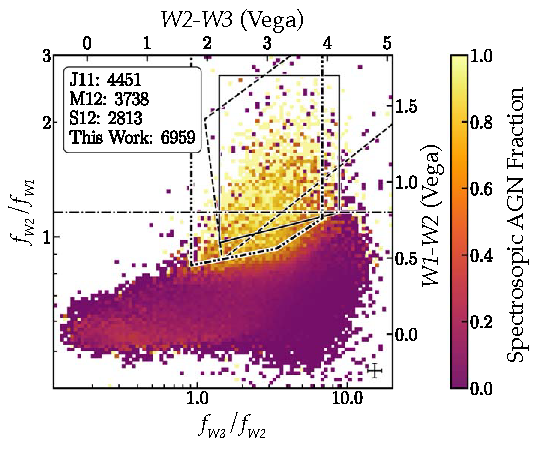
\includegraphics[width=0.8\textwidth]{nuclear/agn_box.pdf}
  \caption[Infrared AGN selection]{AGN Selection based on infrared \textit{WISE} colors. It shows the $W2-W3$ vs. $W1-W2$ color; the fraction of spectroscopically classified AGN is encoded in datapoint color. The dot-dot-dashed box is the one used to flag likely AGN. Adapted from~\cite{Hviding2022}.}
  \labfig{agn_box}
\end{figure}

\subsubsection{MILLIQUAS matching}\label{milliquas_cut}
Additionally to the \textit{WISE} color selection, the MILLIQUAS~\cite{Milliquas} catalog\sidenote{\url{https://quasars.org/milliquas.htm}} was also used to identify likely AGN. This catalog was also used in the regular high-energy neutrino follow-up (see Section~\ref{catmatch}). It contains over 900,000 Type I AGN, roughly 50,000 Type II AGN and again as many quasar candidates.

I was interested in maximizing the purity of the sample in terms of AGN, i.e.~rejecting all likely AGN. Therefore, all objects that had a match in the MILLIQUAS catalog were rejected, regardless of their respective likelihood of the match being an AGN.

\subsection{Adding non-BTS Sources}\label{addsources}
To counter the fact that almost no AGN were present in the BTS sample, forced photometry for an additional 1772 AGN light curves was acquired. This was done by crossmatching sources from a recent AGN study including redshifts~\sidecite{Mechbal2023} with ZTF alerts in a cone with a radius of 3 arcsec. All matched AGN with redshifts available for creating noisified copies were subsequently added to the training sample.

As one of the desired features of the trained classifier was its ability to correctly identify TDEs, it was necessary to increase the number of TDEs in the training sample. For reasons not clear to me, the BTS underperformed significantly in terms of TDE detection rate. To maximize the number of TDEs in the training sample, all published ZTF-detected TDEs were included, resulting in a total number of 66 TDEs available for training the classifier.

\subsection{Creating a less biased Training Sample}
It was not fully possible to control the number of child light curves: There were cases of low-flux objects of which all children failed the signal-to-noise cut. In total, the following number of objects were processed during the training sample augmentation:
\begin{description}
  \item[SNe Ia] The BTS sample contained 3230 SNe Ia, from which 8694 noisified children were created,~i.e. 2.7 children per original light curve on average. The total number of light curves (original ones plus children) was 11924.
  \item[Core-collapse SNe] 1075 CCSNe were available in the BTS sample. With an average of 10.6 children per light curve this amounted to 11,420 children and 12,495 light curves in total.
  \item[AGN] 1893 AGN were originally present. 7177 children were created (3.8 per parent), resulting in 9079 light curves.
  \item[TDE] Starting with 66 TDE, 13,097 children were creating with a large number of children per light curve (198). This amounted to 13,163 light curves in total.
  \item[Stars] As already stated above, stars were not noisified due to their redshift being practically 0. Therefore, only the 525 parent light curves were used, rendering stars the most underrepresented class within the training sample.
\end{description}
Overall, the final training sample contained 47,186 light curves, generated from 6789 initial light curves. On average, $~\sim 6$ child light curves were created from each parent.

\section{Training the Classifier}
In recent years \texttt{XGBoost}\sidenote{\url{https://xgboost.ai}}~\sidecite{Chen2016}, an optimized gradient-boosted decision tree algorithm (this will be explained below), has performed well when classifying structured data; for this reason, it was chosen here.

\subsection{Boosted Decision Trees}
In a regular decision tree, a set of iterative binary decisions (hence `tree') are employed to decide on the classification of an object. Ensemble methods build upon this concept by either working in parallel by creating multiple decision trees with random subsets of features (random forest) or by working in sequence. The latter method qualifies boosted decision trees, meaning that decision trees are generated and evaluated in sequence. The residual squared errors from the first tree are fed into the second tree, and so on. The final classification then is the (weighted) sum of all individual tree's classifications. This method can be generalized to differentiable loss functions in general. If one uses the negative gradient of the squared error loss function instead of the squared error itself, the method is called gradient boosting. \texttt{XGBoost} is one variant of such a gradient boosting algorithm.

\subsection{Hyperparameter Search}
As is usually the case with such algorithms, there is a number of hyperparameters which determine how \texttt{XGBoost} behaves. \texttt{max\_depth} for example avoids overfitting by restricting the size of individual decision trees, the \texttt{learning\_rate} scales down the results by trees other than the initial tree, and \texttt{n\_estimators} controls the number of trees.

These hyperparameters can be tuned by running a grid search in the parameter space, each time training with a small subset of the full data to speed up the process. The parameters yielding the best result are then used when training the full model with the complete training set. In this work, the best values for 9 hyperparameters were searched by randomly drawing from a grid of parameter combinations for 5000 times. This value was chosen as a compromise between computational feasibility and better sampling of the parameter search space. The grid employed here, as well as the chosen hyperparameters are shown in the appendix in Table~\ref{tab:xgboost_grid_search}.

\subsection{Training Procedure}
After obtaining a classified training sample (BTS light curves, see Section~\ref{bts}), AGN and TDE light curves were added (Section~\ref{addsources}) and the sample was augmented and enlarged by creating redshifted and noisified copies (Section~\ref{noisification}). After this, the full training sample was fit with SALT2~(Section~\ref{salt}) and a TDE model (Section~\ref{tde_model}), as well as analyzed with a Bayesian block algorithm (Section~\ref{bayesian_blocks}) to extract features.

The set of features used for training was the following:

\begin{description}
  \item[Peak magnitude] This is the peak observed magnitude (in any filter). The value was scaled accordingly for the noisified and redshifted child light curves:
        \begin{subequations}
          \begin{eqnarray}
            m_\text{child} &=& m_\text{parent} - \mu­_\text{parent} + \mu_\text{child}~~\text{and}\\
            \mu &=& 5(\log_{10}D_L(z)+1),
          \end{eqnarray}
        \end{subequations}
        where $m$ is the parent or child magnitude, $\mu$ is the distance modulus, and $D_L$ is the luminosity distance for redshift $z$.
  \item[SALT2 Fit Results] This included the SALT2 fit parameters $x_0$, $x_1$ and $c$, as well as the reduced $\chi^2$, the non-reduced $\chi^2$ and the degrees of freedom.
  \item[TDE Fit Results] The best-fit TDE Model parameters were also included. These were the rise- and decay times, the peak temperature, the temperature change and the amplitude. The temperature change cutoff time was not included, as the model never picked up on this parameter. The results used also included the $\chi^2$ and the degrees of freedom.
  \item[Overlapping blocks] The number of overlapping regions, extracted with the Bayesian block analysis, was also included to allow identification of non-repeating flares (in contrast to stochastic AGN behavior).
  \item[\textit{WISE} colors] To identify likely AGN, the $W1-W2$ and $W2-W3$ colors of the parent host were  added.
  \item[\texttt{sgscore}] The \texttt{sgscore} of the parent light curve, based on machine learning with PS1 photometry (see Section~\ref{ztf_image_subtraction}), was included as a proxy for host galaxy photometry and morphology.
  \item[Core distance] The median core distance was also included. To account for the fact that the core distance of the redshifted child light curves changed with respect to their parents, this value was recalculated for all children. This was done according to
        \begin{equation}
          \theta_\text{child} = \theta_\text{parent} \frac{D_L(z_\text{parent})}{D_L(z_\text{child})} \frac{(1+z_\text{child})^2}{(1+z_\text{parent})^2},
        \end{equation}
        where $\theta$ is the angular core distance of the child or parent light curve, $D_L$ is the luminosity distance and $z$ is the respective redshift.
\end{description}

\section{Evaluating the Model}
A large fraction of the nuclear sample was unclassified---this is why a classifier was needed in the first place. Therefore, evaluating the classifier's performance needed to happen with a part of the BTS training set. This was done in the usual way: A certain fraction (here: \SI{30}{\percent}) of the training set was kept aside, never to be seen by the classifier beforehand. Such a sample is called a test set.

One pitfall needed to be avoided: The model might learn features of a noisified test light curve by having already seen its parent or one of its siblings in the training process, thereby cheating. To deal with this, the parent light curve and all of its children were always kept together: If e.g.~one child light curve was part of the training set, so were its parent and all its siblings.

\subsection{Performance}
We are now ready to see how the model performs. This is done by first investigating the feature importance, and then by evaluating the confusion matrices.

\subsubsection{Feature Importance}
Feature importance can be used to decide on the usability of certain features, i.e. if they actually contribute to the final classification in a meaningful way. In this study, it was calculated by using a `gain' metric. In this metric, one calculates the average improvement in loss when adding that feature to a tree during training, splitting one branch into two, which could result in more accurate predictions than the original branch.

As one can see in Fig.~\ref{fig:feature_importance}, the feature importance looks well-behaved. The feature importance was distributed fairly equally, as there was not one dominating feature. A dominant feature would raise concerns, as it could be indicative of the classifier finding a loophole regarding the actual task. Also, there were no features present that did not influence the classification at all.

\begin{figure}[htpb]
  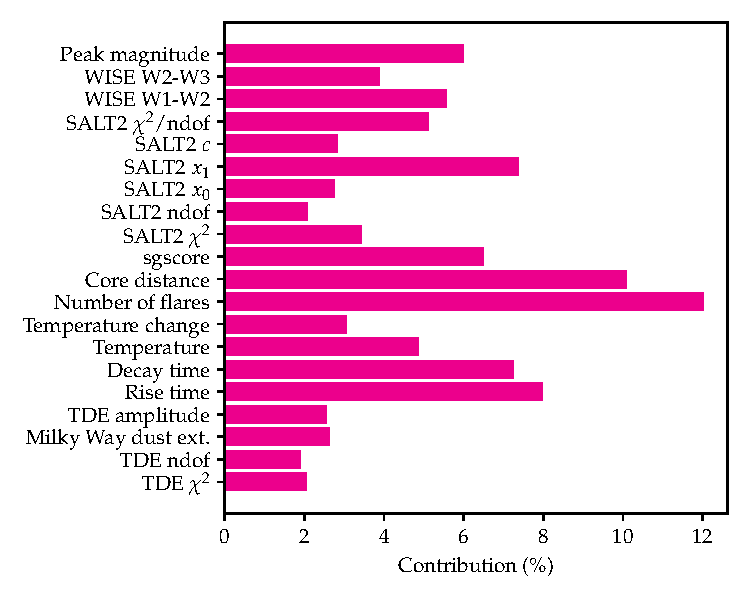
\includegraphics[width=0.6\textwidth]{nuclear/confusion/feature_importance_niter_5000_nsample_2000.pdf}
  \caption[Feature importance]{Feature importance for the classifier when trained with the augmented BTS sample. The relative contribution of each feature to the model is shown in percent, with all individual features adding up to \SI{100}{\percent}.}
  \labfig{feature_importance}
\end{figure}

The two most important features were the number of flares identified by the Bayesian block algorithm, as well as the core distance. This is not surprising, as the former is a good predictor for AGN behavior, and the latter might help in differentiating between AGN/TDEs and supernovae and stars.

Also important were the TDE fit rise- and decay time, as well as the SALT2 fit $x_1$ parameter, which encodes the stretch of the light curve. On equal footing were the peak magnitude and the \texttt{sgscore}. The \textit{WISE} colors were also signficant, as the classifier probably captured the importance of \textit{WISE} colors for AGN classification.

Interestingly, the temperature change did not seem to play a major role, and also the peak temperature was less important as one would have expected from previous studies (see e.g.~\cite{Velzen2021a}). This is indicative of the TDE model fit not capturing all physically present information. It has been shown that a $g-r$ color close to 0, as well as the absence of light curve color evolution are good predictors for TDEs. As the blackbody temperature and temperature change should in principle encode color and color evolution, it is somewhat surprising that these two features do not mirror the importance of color information.

\subsubsection{Confusion Matrices}\label{confusion_matrices}
To see how the model performs with regard to the test set, one can either evaluate a version of the test set also containing child light curves created by the augmentation process, or evaluate only using light curves. There was no reason to favor one method over the other, so both evaluations were performed.

\subsubsection{Test without Augmented Light Curves}
The results from only allowing `real' light curves (i.e.~parent light curves) can be seen in Fig.~\ref{fig:confusion_nonoise}.

\begin{figure}[htb]
  \centering
  \begin{subfigure}[b]{0.49\textwidth}
    \centering
    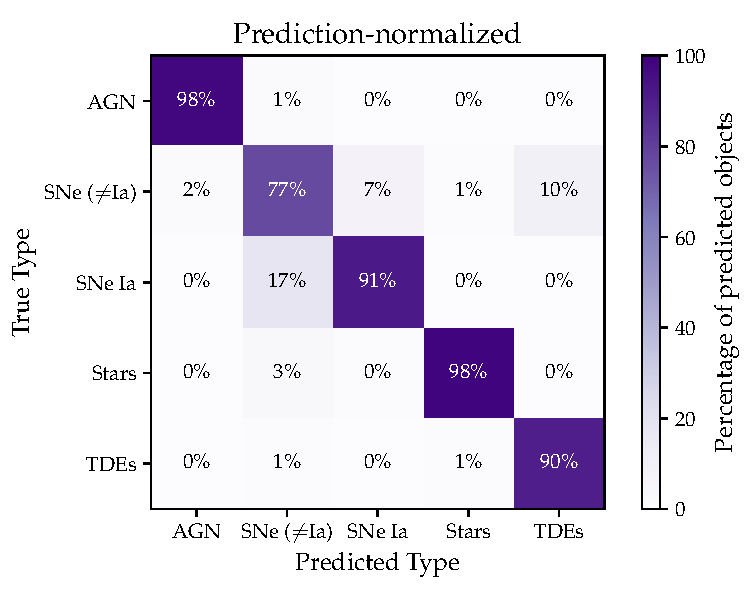
\includegraphics[width=1\textwidth]{nuclear/confusion/results_seed_10_n_iter_5000_noisified_val_False_normaliz_pred.pdf}
  \end{subfigure}
  \begin{subfigure}[b]{0.49\textwidth}
    \centering
    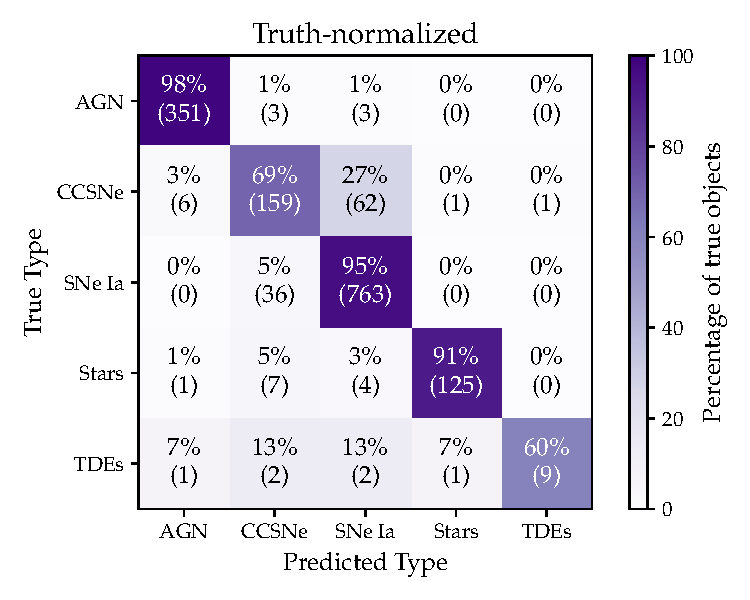
\includegraphics[width=1\textwidth]{nuclear/confusion/results_seed_10_n_iter_5000_noisified_val_False_normaliz_true.pdf}
  \end{subfigure}
  \caption[Confusion matrices without augmentation]{Confusion matrices of the test set predictions, excluding child light curves from the augmentation process. For each figure, the row corresponds to the true type, and the column to the predicted type of object. The matrix on the left shows prediction-normalized values, while the matrix on the right shows truth-normalized values. Absolute numbers are included below the percentages.}
  \labfig{confusion_nonoise}
\end{figure}

As one can see, the absolute numbers displayed in brackets in Fig.~\ref{fig:confusion_nonoise} show that the test set---like the training set---is heavily biased towards SNe Ia, and only 15 TDEs are present.

The left matrix shows the prediction-normalized values: Each number is the percentage of the predicted classifications actually belonging to the predicted class. For example the purity\sidenote{Purity describes how many of the selected objects are in fact TDEs. This metric is also known as `precision' in ML literature} of the TDE selection is \SI{90}{\percent}, meaning 9 out of 10 predicted TDEs are actually TDEs, while the remaining \SI{10}{\percent} are CCSNe in truth. In short, these \SI{10}{\percent} constitute the false positive rate.

The truth-normalized matrix on the right shows the percentage with which objects that in truth belong to a class are correctly identified as members of that class. For example, the TDE completeness\sidenote{Completes details how many of the true class members are identified by a classifier; also known as `recall' in the ML literature.} is \SI{60}{\percent}: 9 out of 15 TDEs were correctly identified as TDE, but \SI{7}{\percent} were misclassified as AGN, \SI{13}{\percent} were wrongly identified as SNe Ia, \SI{13}{\percent} as CCSNe, and \SI{7}{\percent} as stars. The sum of all misclassifications, in this case \SI{40}{\percent}, corresponds to the false negative rate for TDE classification.

The performance looks decent, especially the false positive rate: Except for CCSNe, all predictions capture the truth in \SI{\geq90}{\percent} of all cases. Also, the TDE identification works fairly well: \SI{60}{\percent} of all TDEs were identified by the classifier as such, and of the 10 objects predicted to be TDEs, only 1 was not a TDE. The validity of this result is of course limited by the small number of TDEs in the test sample. As the number of available ZTF light curves of confirmed TDEs is only in the double digits, there is no straightforward fix for this problem.

\subsubsection{Test with Augmented Light Curves}
The evaluation above was repeated, but this time including child light curves from the augmentation process. The results can be seen in Fig.~\ref{fig:confusion_noise}.

The sample looks more balanced due to the inclusion of more noisified child light curves for underrepresented classes (except stars). As one would expect, the overall performance does increase when compared to the test set without child light curves: \SI{97}{\percent} of all predicted TDEs were in fact TDEs (compared to \SI{90}{\percent} without augmentation in the test set), and \SI{79}{\percent} of all TDEs were identified as such (without augmentation: \SI{60}{\percent}).

\begin{figure}[htb]
  \centering
  \begin{subfigure}[b]{0.49\textwidth}
    \centering
    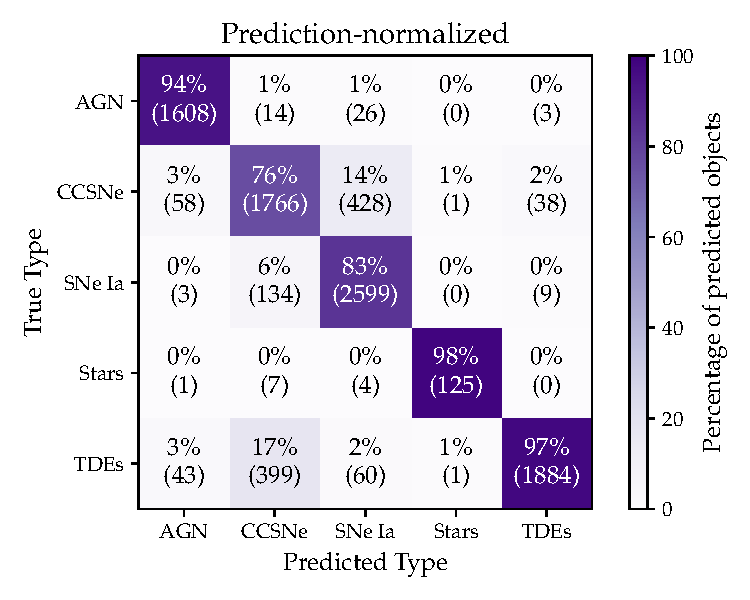
\includegraphics[width=1\textwidth]{nuclear/confusion/results_seed_10_n_iter_5000_noisified_val_True_normaliz_pred.pdf}
  \end{subfigure}
  \begin{subfigure}[b]{0.49\textwidth}
    \centering
    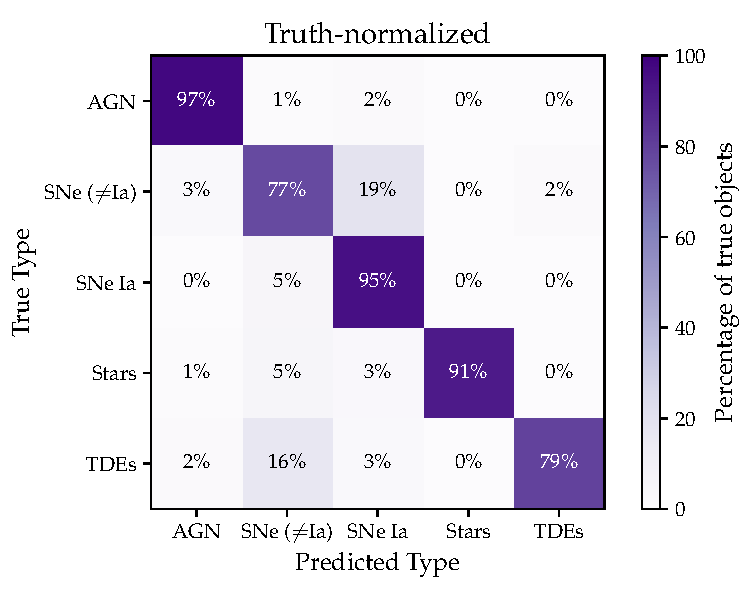
\includegraphics[width=1\textwidth]{nuclear/confusion/results_seed_10_n_iter_5000_noisified_val_True_normaliz_true.pdf}
  \end{subfigure}
  \caption[Confusion matrices with augmentation]{Confusion matrices of the test set predictions, including child light curves from the augmentation process. Left: prediction-normalized; right: truth-normalized.}
  \labfig{confusion_noise}
\end{figure}


\section{Finding Candidate TDEs}\label{visual_cuts}

The traditional method of selecting TDE candidates consists of a sequence of two-dimensional cuts in the fit result parameter space (see e.g.~\cite{Velzen2019}). One way of increasing the purity of the machine-learning selected TDEs is by defining such a set of 2D cuts by studying the BTS sample, and applying the very same cuts to the nuclear sample.

To do this, the classified part of the BTS sample enriched by additional TDEs was evaluated with exactly the same features as used in the training of the classifier model. The goal was to look for a set of cuts in the fit parameter space that would retain a high number of TDEs, while rejecting as many non-TDE as possible.

\subsection{2D Cuts: Different Cut Stages}
An overview over the sample after subsequent application of these two-dimensional cuts, as well as the TDE selection purity and completeness can be seen in Figure~\ref{fig:bts_scatter}. These were the stages (the numbers in brackets correspond to the individual plots, with (1a) showing the sample without cuts):

\begin{description}
  \item[AGN Veto (1b, 2a)] Although the BTS is already biased against AGN, the BTS sample still contained objects which could be ruled out as likely AGN by crossmatching to MILLIQUAS (1b) and selecting based on \textit{WISE} colors (2a), see Section~\ref{agn_rejection}.
  \item[Core distance (2b)] As the BTS is not selecting nuclear transients per se, nuclearity needed to be enforced by requiring a maximum core distance of \SI{0.4}{\arcsec}.
  \item[\texttt{sgscore} cut (3a)] Only transients with an \texttt{sgscore} $<0.3$ were allowed at this cut stage.
  \item[SNIa diagonal cut (3b)] The transient had to be to the right side of a diagonal cut in the rise decay time plane, described by $3.55 - 2.29 \tau$ (with $\tau$ being the decay time, all values in $\log~\text{day}$).
  \item[Temperature cut (4a)] The temperature was required to lie between $\log \SI{3.9}{\K}$ and $\log\SI{4.4}{\K}$. Furthermore, the daily temperature change $\Delta T$ was required to lie between $\SI{-100}{\K\per\deh} < \Delta T < \SI{150}{\K\per\deh}$ (left).
  \item[Rise- and decay-time cut (4b)] The rise and decay times were required to lie within $\log \SI{0.8}{\deh} < \text{risetime} < \log \SI{2.05}{\deh}$ and $\log \SI{1.1}{\deh} < \text{decaytime} < \log \SI{3.0}{\deh}$.
  \item[$\chi^2$ cut (5a)] Only those transients with a TDE fit reduced $\chi^2$ outperforming their SALT2 fit reduced $\chi^2$ were selected here to reject remaining likely SNe Ia. Also, the reduced TDE fit $\chi^2$ was required to lie below 6.
  \item[Exactly one flare (5b)] Finally, only transient with a single flare coincident in \textit{g}- and \textit{r}-band were allowed to reject likely stochastic AGN activity.
\end{description}

\subsection{Visual Cuts: Evaluate the Cuts}
Before all cuts, only requiring the TDE model fit to succeed, the sample consistsed of 4094 transients, of which 64 were TDEs. This corresponded to an initial purity of \SI{1.6}{\percent} and a selection completeness of \SI{100}{\percent} (all TDEs are of course retained before any cuts).

\subsubsection{All Cuts Combined}
The final selection consisted of 39 transients, of which 31 were TDE. This translates to a purity of \SI{79.5}{\percent}, with a selection completeness of \SI{48.4}{\percent}, i.e.~roughly half of the TDE survive all cuts.
The purity and completeness with subsequent cut stages are shown in Fig.~\ref{fig:completeness_purity}.

\begin{figure}[htpb]
  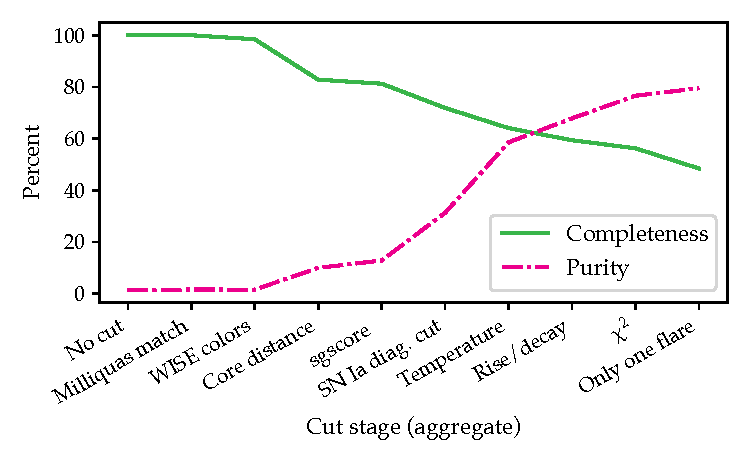
\includegraphics[width=1\textwidth]{nuclear/completeness_purity.pdf}
  \caption[Visual TDE selection]{Completeness (green line) and purity (magenta, dash-dot) of the visual TDE selection. The cut stages are shown on the x-axis, with each new cut added on top of all previous cuts.}
  \labfig{completeness_purity}
\end{figure}

These numbers were somewhat promising, as objects lying within the final selection had a 4 in 5 chance of correctly being identified as TDE while only sacrificing half of the TDE population. Of course, there is always a trade-off between completeness and purity; i.e. a program designed to discover TDEs early on might need to accept a lower purity.

\begin{figure}[htbp]
  \centering
  \begin{subfigure}[b]{0.49\textwidth}
    \centering
    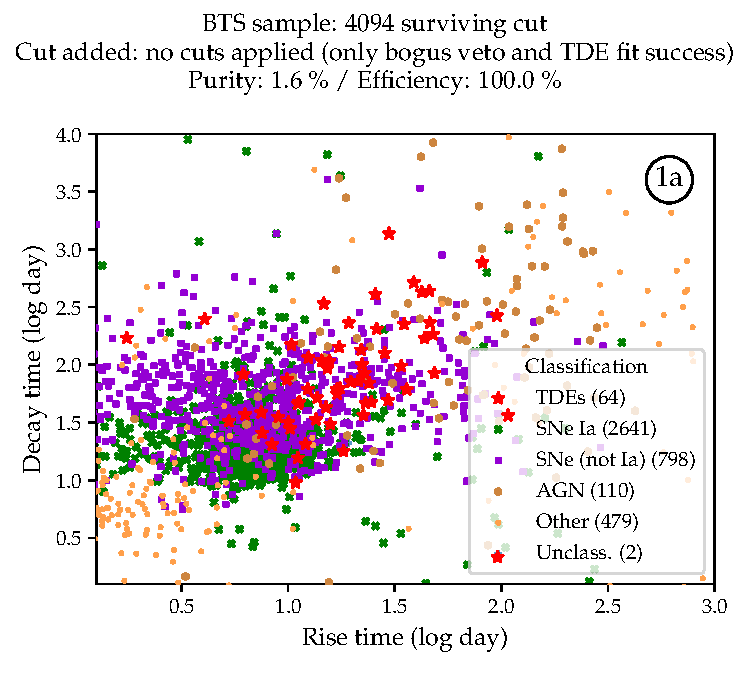
\includegraphics[width=1\textwidth]{nuclear/scatter/tde_rise_decay_['nocut'].pdf}
  \end{subfigure}
  \begin{subfigure}[b]{0.49\textwidth}
    \centering
    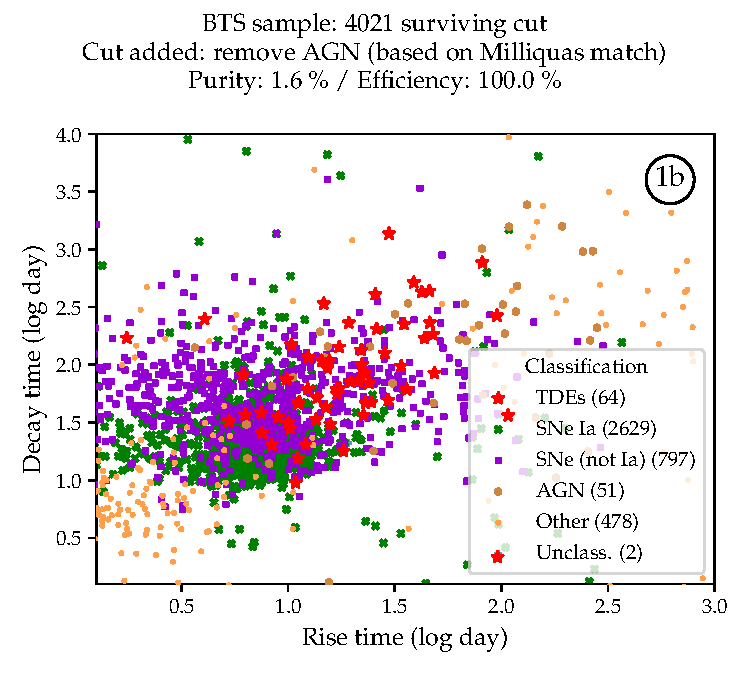
\includegraphics[width=1\textwidth]{nuclear/scatter/tde_rise_decay_['nocut', 'milliquas_noagn'].pdf}
  \end{subfigure}
  \begin{subfigure}[b]{0.49\textwidth}
    \centering
    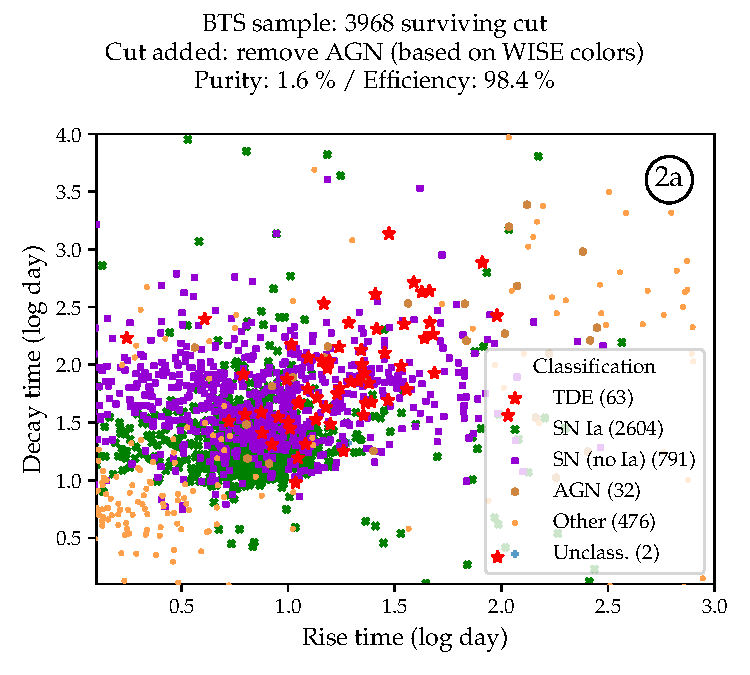
\includegraphics[width=1\textwidth]{nuclear/scatter/tde_rise_decay_['nocut', 'milliquas_noagn', 'wise_noagn'].pdf}
  \end{subfigure}
  \begin{subfigure}[b]{0.49\textwidth}
    \centering
    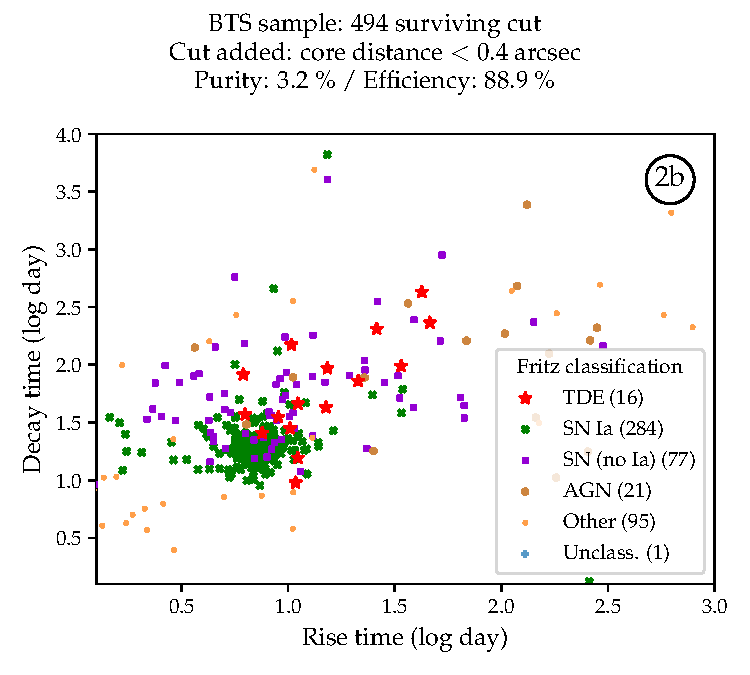
\includegraphics[width=1\textwidth]{nuclear/scatter/tde_rise_decay_['nocut', 'milliquas_noagn', 'wise_noagn', 'coredist'].pdf}
  \end{subfigure}
  \begin{subfigure}[b]{0.49\textwidth}
    \centering
    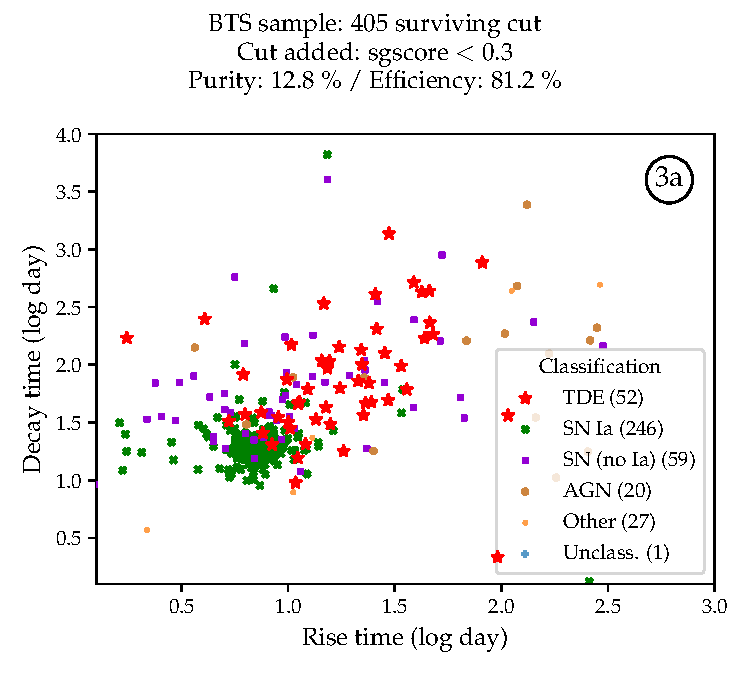
\includegraphics[width=1\textwidth]{nuclear/scatter/tde_rise_decay_['nocut', 'milliquas_noagn', 'wise_noagn', 'coredist', 'sgscore'].pdf}
  \end{subfigure}
  \begin{subfigure}[b]{0.49\textwidth}
    \centering
    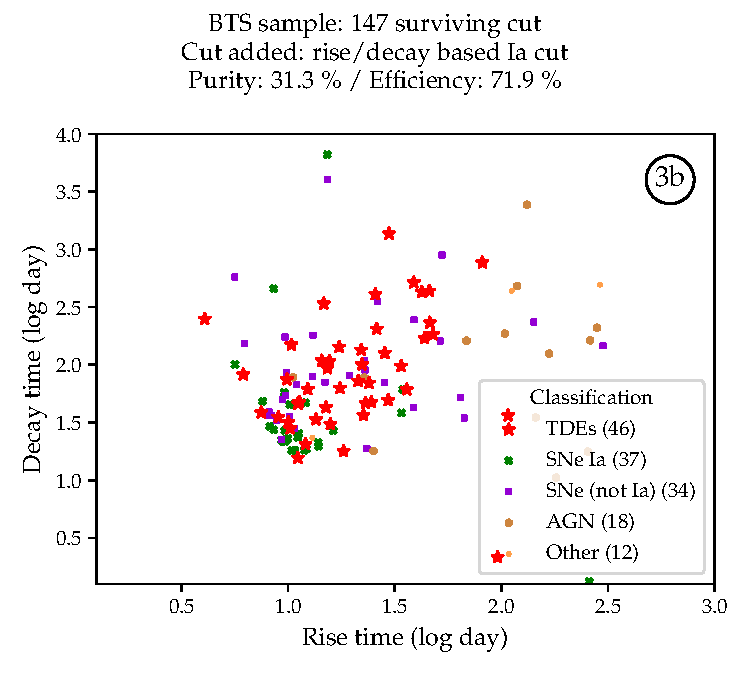
\includegraphics[width=1\textwidth]{nuclear/scatter/tde_rise_decay_['nocut', 'milliquas_noagn', 'wise_noagn', 'coredist', 'sgscore', 'snia'].pdf}
  \end{subfigure}
  \begin{subfigure}[b]{0.49\textwidth}
    \centering
    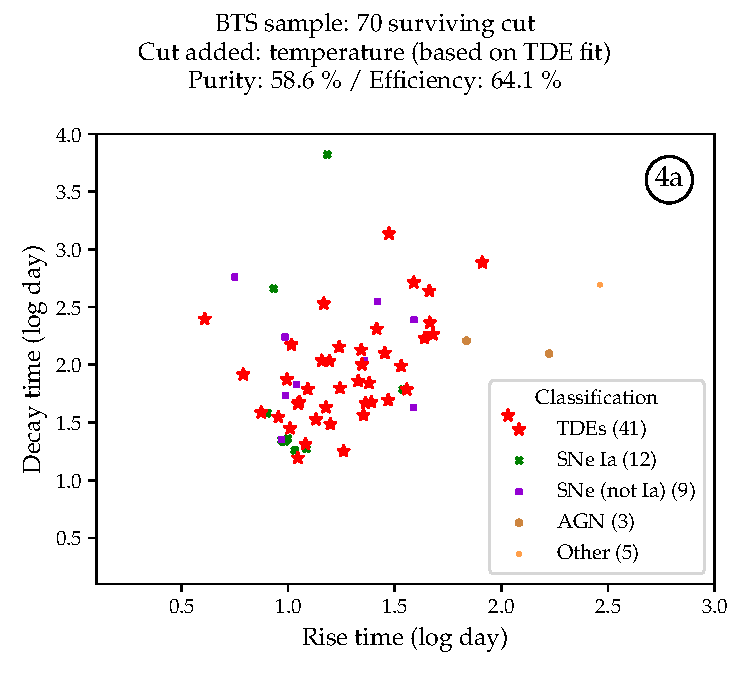
\includegraphics[width=1\textwidth]{nuclear/scatter/tde_rise_decay_['nocut', 'milliquas_noagn', 'wise_noagn', 'coredist', 'sgscore', 'snia', 'temp'].pdf}
  \end{subfigure}
  \begin{subfigure}[b]{0.49\textwidth}
    \centering
    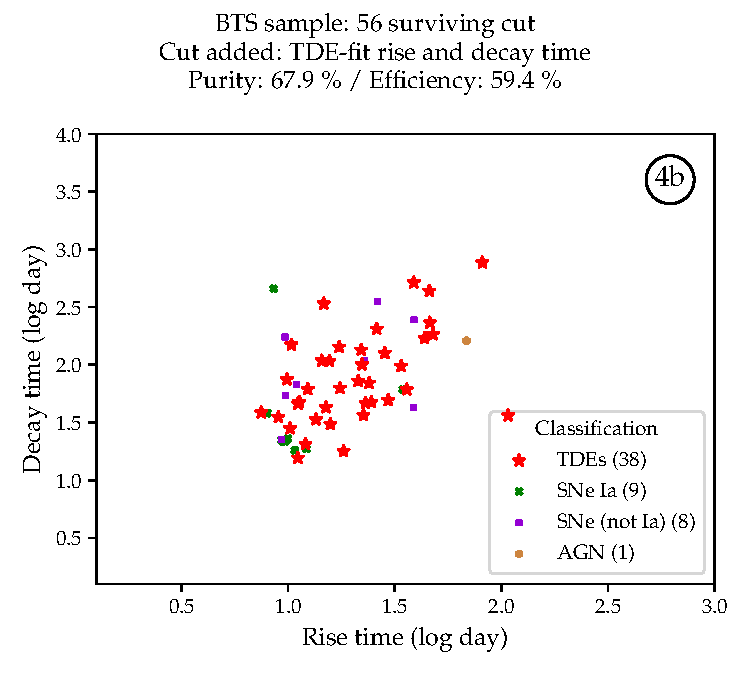
\includegraphics[width=1\textwidth]{nuclear/scatter/tde_rise_decay_['nocut', 'milliquas_noagn', 'wise_noagn', 'coredist', 'sgscore', 'snia', 'temp', 'risedecay'].pdf}
  \end{subfigure}
  \begin{subfigure}[b]{0.49\textwidth}
    \centering
    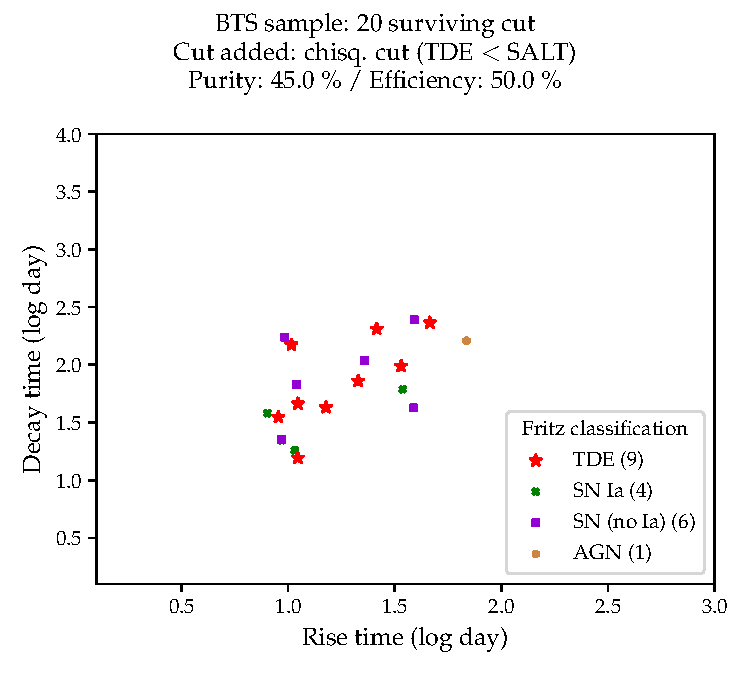
\includegraphics[width=1\textwidth]{nuclear/scatter/tde_rise_decay_['nocut', 'milliquas_noagn', 'wise_noagn', 'coredist', 'sgscore', 'snia', 'temp', 'risedecay', 'chisq'].pdf}
  \end{subfigure}
  \begin{subfigure}[b]{0.49\textwidth}
    \centering
    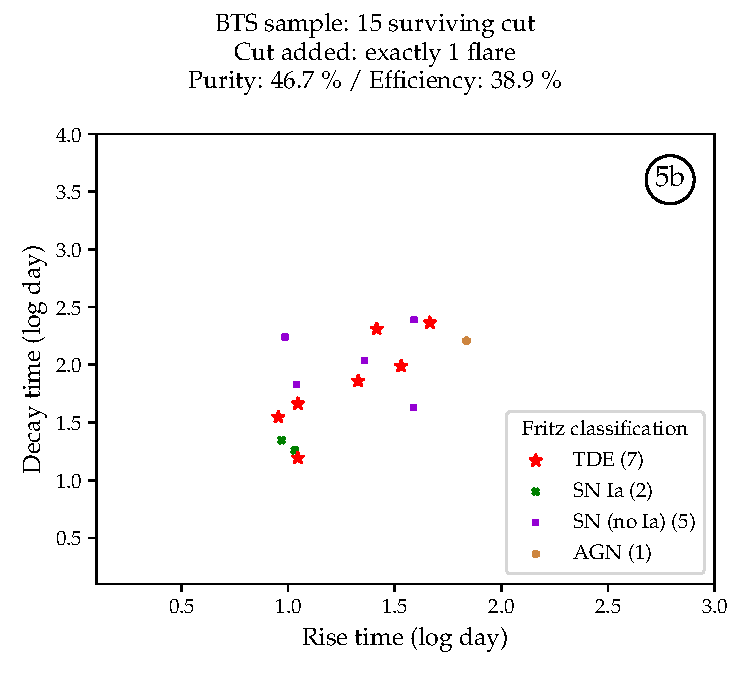
\includegraphics[width=1\textwidth]{nuclear/scatter/tde_rise_decay_['nocut', 'milliquas_noagn', 'wise_noagn', 'coredist', 'sgscore', 'snia', 'temp', 'risedecay', 'chisq', 'bayes'].pdf}
  \end{subfigure}
  \caption[BTS selection]{2D-cut based selection of TDEs among the classified objects of the Bright Transient Survey (augmented with additional TDEs). These are displayed in the rise- and decay-time plane, as derived from the TDE fit (see Section~\ref{tde_model}). From top to bottom and left to right, more and more cuts are added.\newline \newline All classes also used in the training of the classifier are shown. These were TDEs (red stars), SNe Ia (green diagonal crosses), CCSNe (purple squares), AGN (brown hexagons), other types (orange circles), and unclassified objects (blue crosses).\newline \newline Top row: No cuts applied (1a) and the MILLIQUAS-based AGN veto (1b).\newline \newline Second row: AGN cut based on \textit{WISE} colors (2a) and cut based on the core distance (2b).\newline \newline Third row: The \texttt{sgscore} is required to lie below 0.3 (3a) and SNe Ia are removed by a diagonal cut in the rise-/decay time plane (3b)\newline \newline Fourth row: The temperature and temperature evolution were restricted (4a), as were the rise and decay times (4b). \newline \newline Bottom row: Finally, it was required that the TDE model was a better fit than the SALT2 model by requiring the reduced $\chi^2$ of the TDE fit to be smaller than the SALT2 fit's $\chi^2$ (5a), and that the transient light curve had exactly 1 flare (5b).}
  \labfig{bts_scatter}
\end{figure}

After establishing and verifying the 2D cuts, everything is ready to use them on the model predictions and investigate its performance further.

\section{A Photometric TDE sample}
As we now obtained a trained classifier and a set of 2D cuts optimized for isolating TDE candidates, the next step was to classify the nuclear sample with the trained model, and subject it to the very same cuts.

\subsection{Running the Classifier}\label{classifier_res}
The full classification of the nuclear sample is shown in Fig.~\ref{fig:classification_maghist_nocut}. Here, the plots on top only show non-AGN hosts, while the bottom plots show likely AGN hosts. This differentiation was again achieved by crossmatching to the MILLIQUAS catalog and selecting based on \textit{WISE} colors (see Section~\ref{agn_rejection}). The plots on the left show community classifications drawn from Fritz, the GROWTH Marshal and the TNS, while the right side plots display the \texttt{XGBoost} classifications.

\begin{figure}[H]
  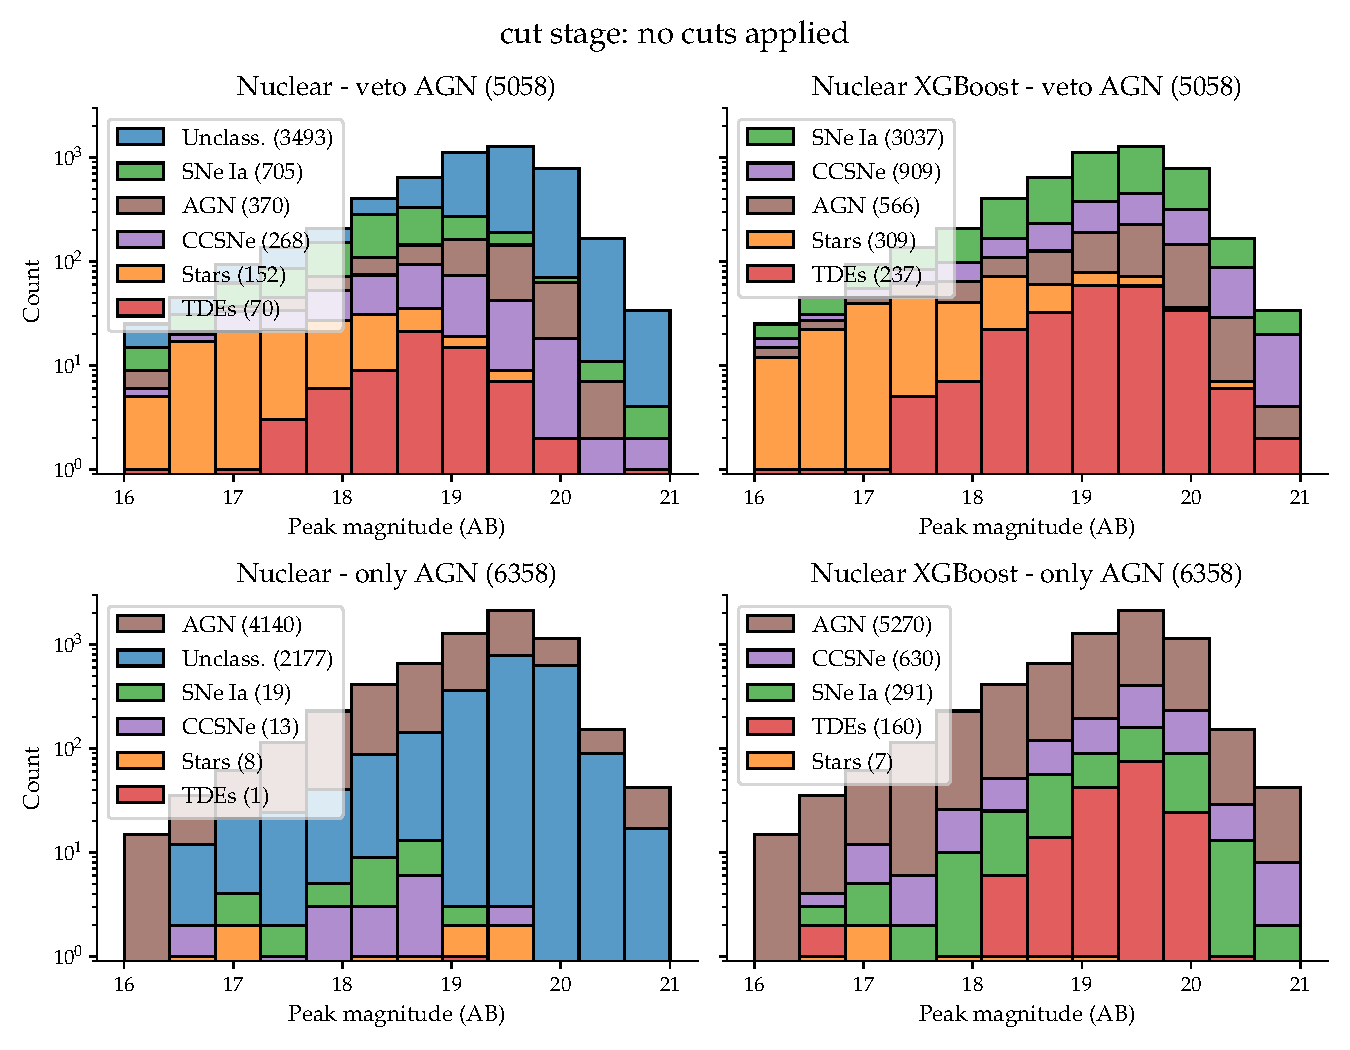
\includegraphics[width=1\textwidth]{nuclear/maghist/maghist_['nocut']_comb.pdf}
  \caption[Classification without cuts]{Classifications of the \texttt{XGBoost} model. This figure shows the nuclear sample, binned in magnitude steps of $0.5$. There are no cuts applied. The classifications on the left side come from the community, i.e.~Fritz, the GROWTH Marshal or TNS. The plots on the right side show the \texttt{XGBoost} classifications. The top row shows non-AGN hosts, while the bottom row shows likely AGN hosts.}
  \labfig{classification_maghist_nocut}
\end{figure}

Looking at the \texttt{XGBoost} classifications of the AGN part of the nuclear sample (bottom right plot), one can notice that---reassuringly---the majority (\SI{83}{\percent}) was indeed classified as AGN by the decision tree. As the non-AGN part of the nuclear sample is much more likely to contain bona fide transients, we will now focus on this selection (top right plot). At this stage, without further cuts on the sample, \texttt{XGBoost} classified 3037 objects as SNe Ia, 909 as CCSNe, 566 as AGN, 309 as stars, and 237 as TDEs.

\begin{figure}[htpb]
  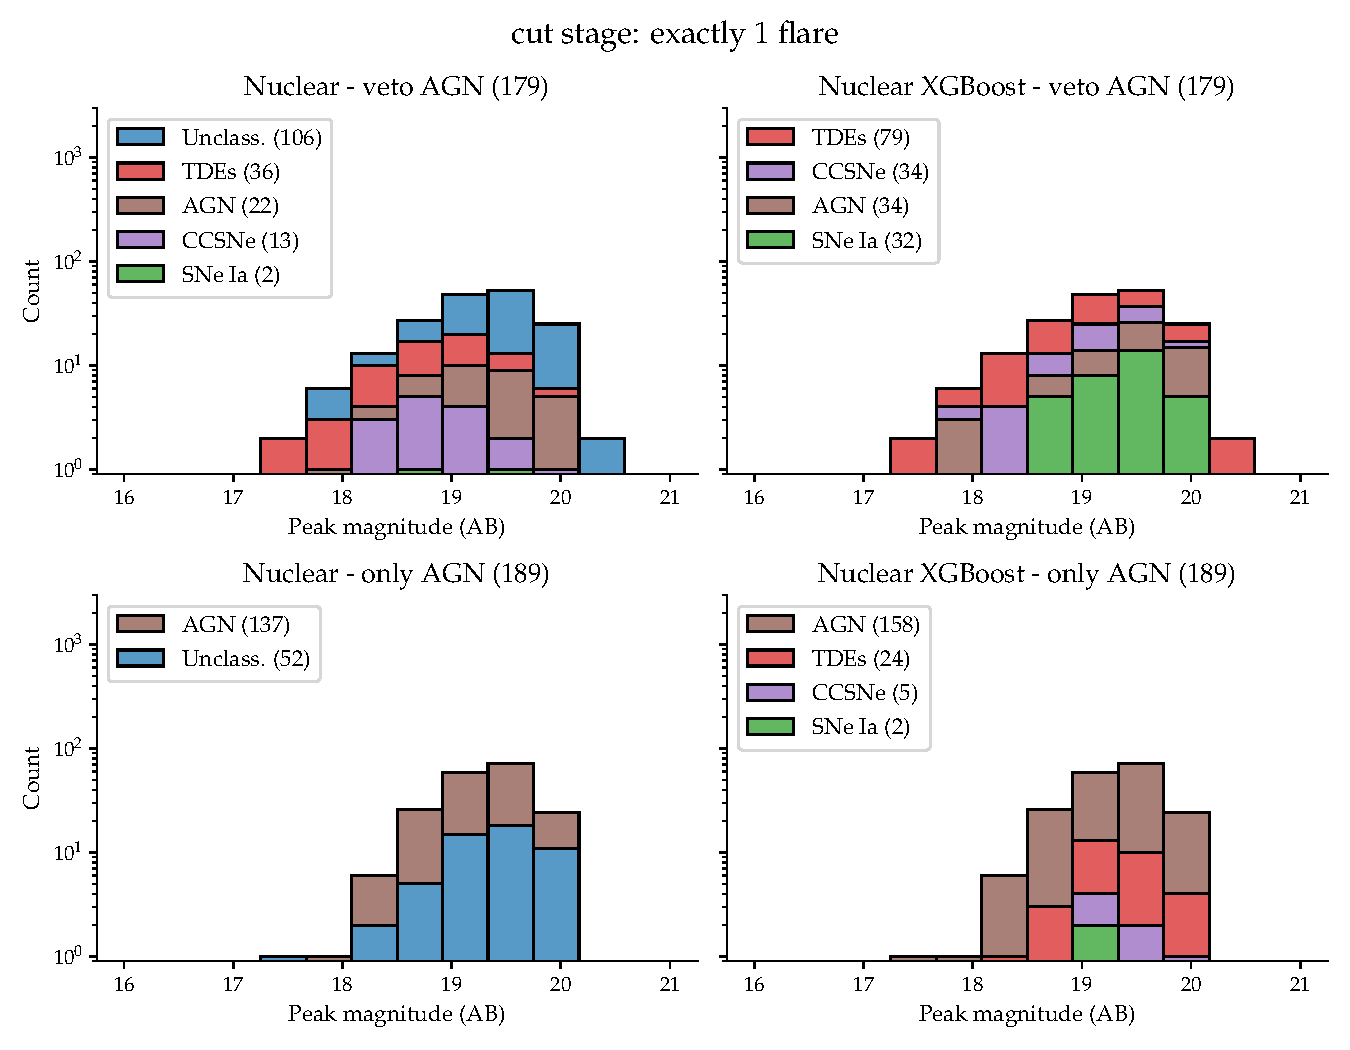
\includegraphics[width=1\textwidth]{nuclear/maghist/maghist_['nocut', 'coredist', 'sgscore', 'snia', 'temp', 'risedecay', 'chisq', 'bayes']_comb.pdf}
  \caption[Classification with all 2D cuts]{Classifications of the \texttt{XGBoost} model, this time with all the 2D cuts applied. Left side: community classifications, i.e. from~Fritz, the GROWTH Marshal or TNS; right side: \texttt{XGBoost} classifications. Top row: non-AGN hosts; bottom row: likely AGN hosts.}
  \labfig{classification_maghist_cut}
\end{figure}

To obtain a purer (but of course less complete) TDE sample, the 2D cuts established in Section~\ref{visual_cuts} were applied. The classification of nuclear sample after application of these cuts can be seen in Fig.~\ref{fig:classification_maghist_cut}. The full list of all 79 transients from non-AGN hosts classified as TDE, including new and already known ones can be found in the appendix, see Table~\ref{tab:tde_candidates}. In total, 27 new TDE candidates could be added to the list of already known and spectroscopically classified TDEs. An overview of the candidates is shown in Table~\ref{tab:tde_candidates} in the appendix.

The 24 objects classified as TDEs that were lying in AGN hosts (Fig.~\ref{fig:classification_maghist_cut}, bottom right plot) were also evaluated. Unfortunately, visual inspection of these events ruled out all but one (\textit{\href{https://ztfnuclear.simeonreusch.com/transient/ZTF18acryjql}{AT2018ktr}}) transient. Visually rejecting the transients was almost always possible based on light curve features alone. This highlights potentially lacking performance of the classifier. On the bright side, this selection shows that the AGN rejection seems to work, as significantly fewer events (24 vs. 79 for the non-AGN hosts) were initially classified as TDEs at that stage.

\subsection{Inspection of Objects Classified as TDE}\label{all_tde_inspection}
One pitfall in evaluating the classifier performance comes from the fact that \SI{70}{\percent} of all TDEs were already seen by the classifier in the training stage---this was necessitated by the fact that there were not many to begin with. Therefore, a visual inspection of all objects classified as TDE that were not already known as TDEs during the training stage was performed.

This was done for the non-AGN part of the sample (see top right histogram in Fig.~\ref{fig:classification_maghist_nocut}). Of the 237 objects classified as TDE, 29 were already seen by the classifier during the training stage and were therefore excluded, leaving 208 transients. These were then visually inspected, and rated according to the following scheme: `Correct' meant that the transient looked like a plausible TDE, and no contrary evidence---like a classification based on a spectrum---existed. `Possible' meant that either the light curve looked ambiguous, or the TDE fit result looked unsatisfying (for example, unphysically fast rise and fade timescales), but a clear misclassification could be excluded. Finally, `wrong' was reserved for transients where the visual inspection rendered the TDE-classification unlikely, as e.g.~stochastic AGN variability was present.

The exact rejection reasons for judging classifications as `wrong' were: Misclassification based on an available spectrum, issues with the light curve quality, the existence of multiple recurring flares within the light curve, the existence of only one flare, but paired with a variable baseline suggestive of AGN variability, and finally not a clear flare, but only slightly elevated flux above a variable baseline. A breakdown of all 93 transients discarded due to these reasons is given in Table~\ref{tab:rejection_statistics}, while an example for each category in that Table is shown in Fig.~\ref{fig:rejection_examples}.

\begin{table}
  \centering
  \def\arraystretch{1.2}
  \begin{tabular}{c c  c  c c}
    \hline
    \textbf{Spectrum says} & \textbf{Data}    & \textbf{Multiple} & \textbf{1 flare, but}      & \textbf{No}    \\
    \textbf{no TDE}        & \textbf{quality} & \textbf{flares}   & \textbf{variable baseline} & \textbf{flare} \\
    \hline
    \hline
    16                     & 4                & 24                & 26                         & 23             \\
    \hline
  \end{tabular}
  \caption[Visual inspection: rejection statistics]{Rejection statistics for the visual inspection of the 93 transients analyzed and rated as `wrong classification'.}
  \label{tab:rejection_statistics}
\end{table}

\begin{figure}[htbp]
  \centering
  \begin{subfigure}[htb]{0.48\textwidth}
    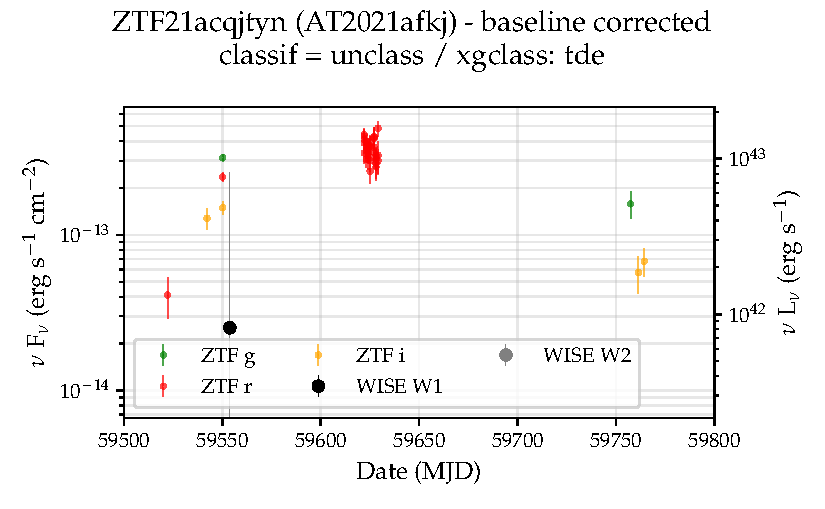
\includegraphics[width=1\textwidth]{nuclear/rejection/ZTF21acqjtyn.pdf}
  \end{subfigure}
  \begin{subfigure}[htb]{0.48\textwidth}
    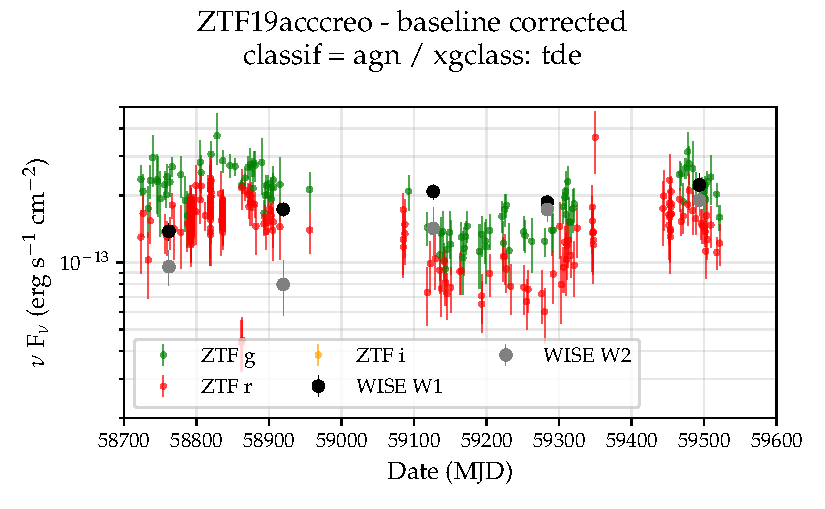
\includegraphics[width=1\textwidth]{nuclear/rejection/ZTF19acccreo.pdf}
  \end{subfigure}
  \begin{subfigure}[htb]{0.48\textwidth}
    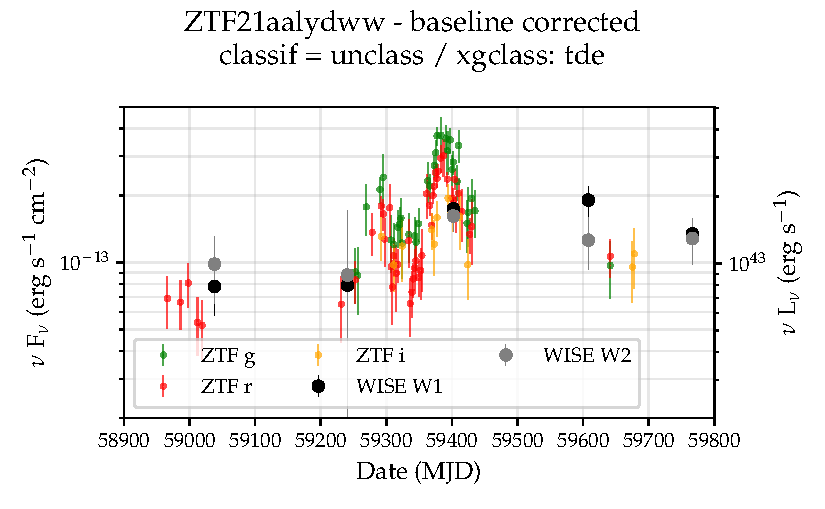
\includegraphics[width=1\textwidth]{nuclear/rejection/ZTF21aalydww.pdf}
  \end{subfigure}
  \begin{subfigure}[htb]{0.48\textwidth}
    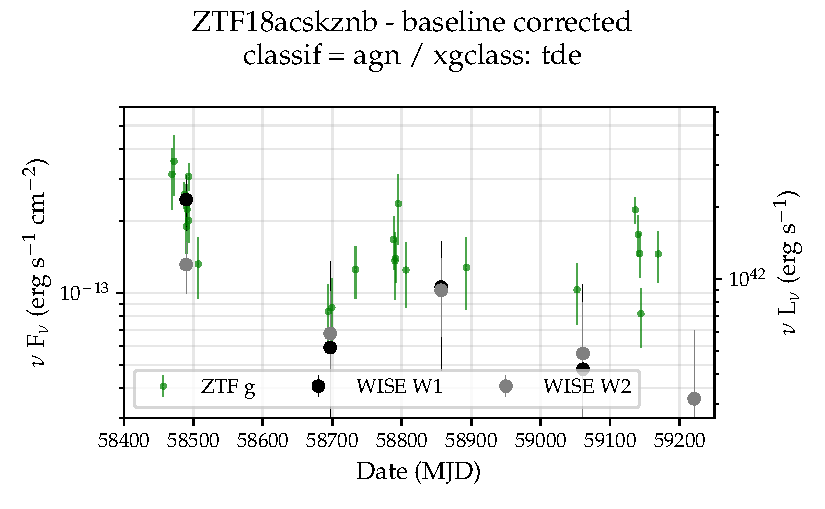
\includegraphics[width=1\textwidth]{nuclear/rejection/ZTF18acskznb.pdf}
  \end{subfigure}
  \caption[Examples of visual AGN rejection]{Examples for the different categories of visual AGN rejection. Top left: Data quality issues. Top right: There were multiple flares, which the Bayesian block algorithm failed to detect. Bottom left: Only one clear flare was detected, but there were signs of a variable baseline. Bottom right: No flare was discernible.}
  \labfig{rejection_examples}
\end{figure}

Of the 208 transients thus analyzed, 82 had a correct classification, for 33 a TDE nature was possible, and 93 were rated as wrong, i.e. misclassifications. When one generously rates both `correct' and `possible' as correct classification, a false positive rate of \SI{44.7}{\percent} results. If one is more conservative and counts `possible' as misclassification, a false positive rate of \SI{60.5}{\percent} ensues.

In any case, these numbers mark a sharp drop compared to the \SI{10}{\percent} false positive rate for the augmented BTS test sample (see Section~\ref{confusion_matrices}). This gets alleviated a bit by the fact that TDEs which were present during the training phase were excluded---so the `real' performance might as well be better. One can therefore safely assume that roughly half of the transients classified as TDE are in fact TDEs. All further calculations will be done with the assumption of a \SI{50}{\percent} false positive rate.

On the bright side: Many of the clear misclassifications showed signs of AGN baseline variability. As can be seen in Table~\ref{tab:rejection_statistics}, 24 transients showed multiple flares, and 23 showed only slightly elevated flux above a variable baseline. It should be possible to develop a second classifier designed only to discern these features. If that were possible, the false positive rate could be reduced to roughly \SI{22}{\percent}.

\subsection{Conclusions for Photometric Classification}
The performance of the classifier yielded somewhat mixed results. There was a number of problems identified that need to be addressed to improve the classification quality:

\begin{description}
  \item[Data quality] In some cases, inspection of transients classified as TDE showed a sparsely sampled light curve, e.g.~\textit{\href{https://ztfnuclear.simeonreusch.com/transient/ZTF21aanubdr}{ZTF21aanubdr}}. A human would recognize that the sparse sampling allowed only little conclusions to be drawn, while the decision tree had no adequate way of reacting to that fact. It would be beneficial to somehow infer from the data quality the range of conclusions that could possibly be drawn for a specific object.
  \item[Misclassifications] There were examples where visual inspection allowed for easy and straightforward classification---especially in the case of stochastic AGN variability---but the classifier struggled to identify the AGN-nature of the transient. This highlights that there might still be room for improvement, i.e.~further features that humans easily grasp and which could be exploited for automatic classification. The `exactly 1 coincident flare' feature was apparently not sufficient for this task, and neither was a high reduced $\chi^2$ of the TDE and SALT2 fits. It should be possible to add another classifier designed just to identify periodic features typical for such stochastic AGN behavior.
  \item[Effectiveness of Augmentation] The TDE classification performance of the classifier when applied to the nuclear sample was investigated in Section~\ref{all_tde_inspection}. The results were worse than the confusion matrices of the test sample (see Section~\ref{confusion_matrices}) suggested: At least 101 of 208 objects classified as TDE and not seen by the classifier during training are most likely something else, resulting in a much higher false positive rate (\SI{48.5}{\percent}) than the test sample suggested. This means that the augmentation by creating redshifted and noisified copies was not able to fully capture the transition from the BTS sample to the fainter nuclear sample.
\end{description}

\section{Selection by Dust Echo}\label{dustecho_sel}
Another avenue explored for obtaining interesting and hitherto missed nuclear transients was a selection based on their infrared dust echo. For this, all transients with a \texttt{T2DustEchoEval} result (see Section~\ref{irdata}) suggesting the existence of an infrared flare occurring simultaneous to or after the optical peak were visually inspected.

\subsection{Inspection Tool}
To aid in the visual inspection of light curves, I created a web-based frontend to interactively view the light curves of the nuclear sample, especially the ones showing an infrared flare qualifying for a dust echo. This tool, accessible under \url{https://ztfnuclear.simeonreusch.com}, was written in Python. It is based on the \texttt{Flask}\sidenote{\url{flask.palletsprojects.com}} web framework, and operated behind an \texttt{nginx} web server also serving as reverse proxy, hosted on a virtual private server.

Fig.~\ref{fig:ztfnuclear_frontend} shows the frontend. It was designed to display the transient light curve, results from the crossmatching, a redshift if one was found, as well as links to object pages on the GROWTH Marshal, Fritz and TNS. Lastly, it offered the functionality to leave comments (this is why a login system was created) and to rate the transient as `interesting', `maybe interesting', and `boring'.

\begin{figure}[htb]
  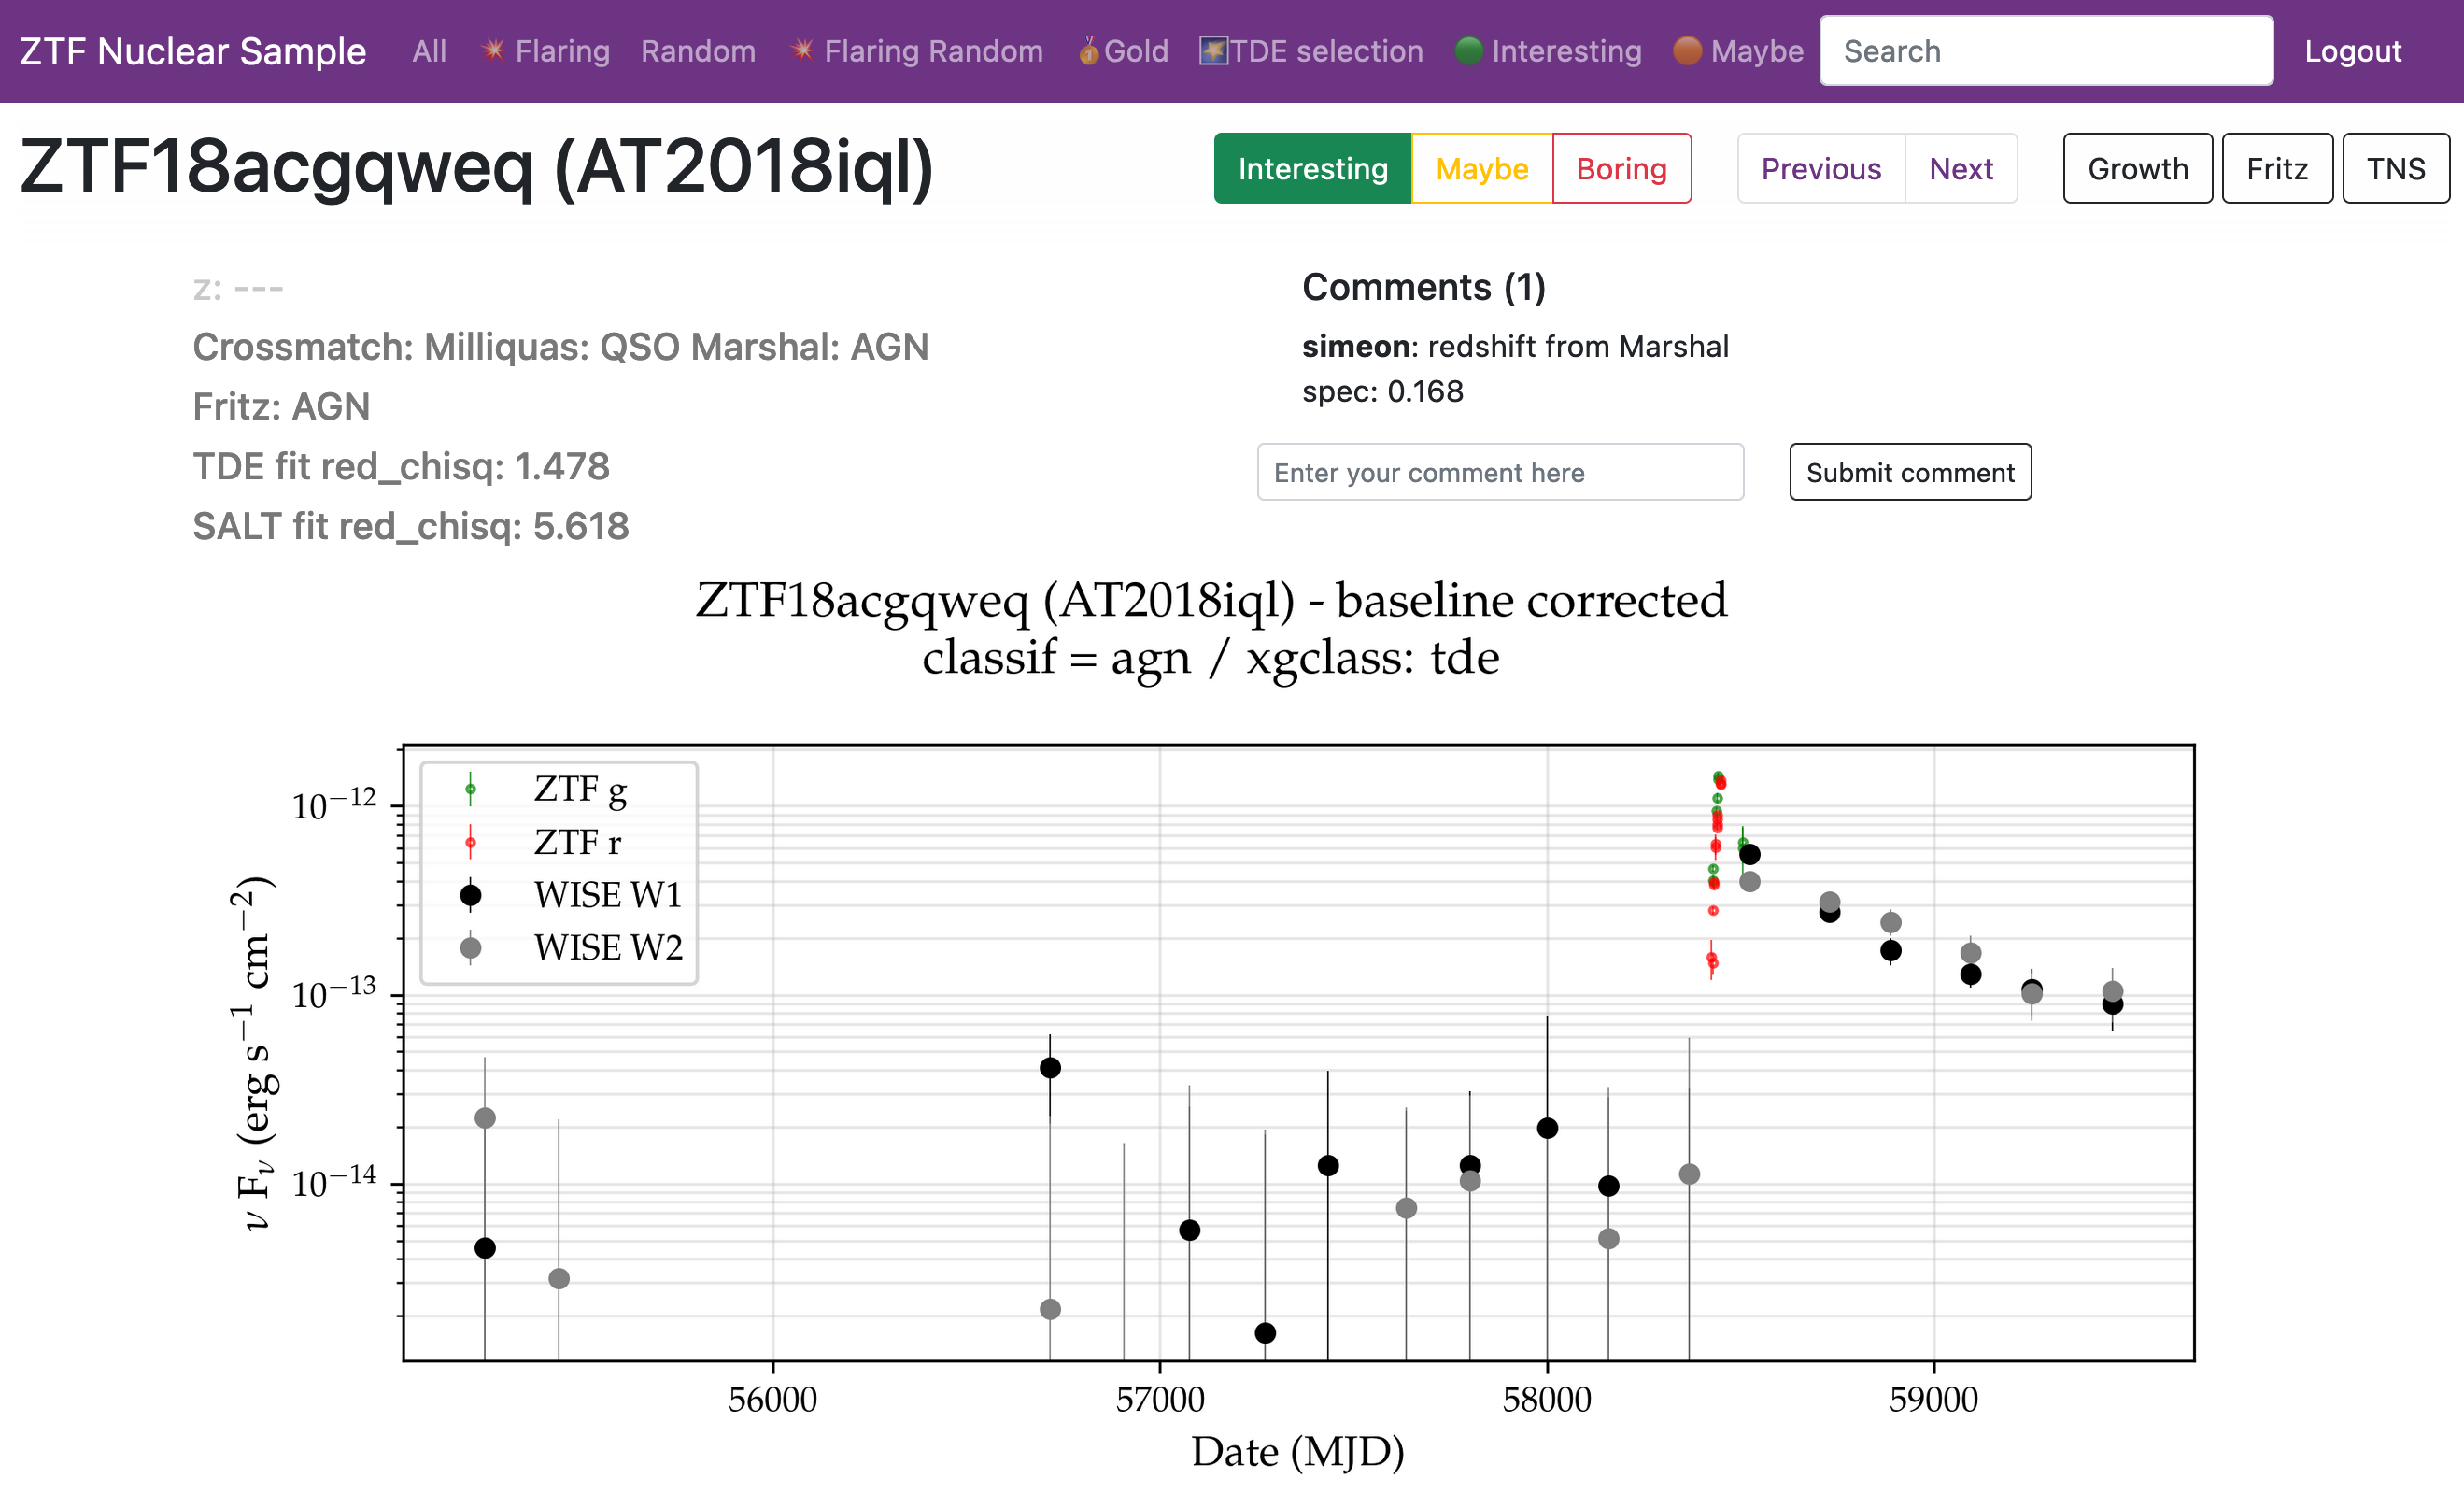
\includegraphics[width=1\textwidth]{nuclear/ztfnuclear_frontend.png}
  \caption[Frontend for the nuclear sample]{The frontend for inspecting and reviewing the nuclear sample. It shows an exemplary page for \textit{\href{https://ztfnuclear.simeonreusch.com/transient/ZTF19abqyosy}{ZTF19abqyosy}}, including a light curve, a comment and a rating as `Interesting'. The fit results of the TDE and the SALT2 fit are displayed as well, plus potential redshift matches (none in this case).}
  \labfig{ztfnuclear_frontend}
\end{figure}

\subsection{Creating a Dust Echo Sample}
To create a sample of dust echo transients that looked promising, multiple users reviewed all transients with a \texttt{T2DustEchoEval} score of 1, designed to select infrared flares compatible with stemming from a dust echo. A dust echo evaluation score of 1 selects those infrared flares which have a reliable baseline in both bands before the flare, and for which the flare is evolving reasonably fast (rise time $<1000$ days, fade time $<5000$ days).

The review was performed using the web frontend, and each user rated the transients as either `interesting', `maybe interesting' or `boring'. The final selection comprised transients that were rated as `interesting' by at least two users. An overview over the 37 transients that met this criterion can be found in the appendix in Table~\ref{tab:dustecho_selection}.

\subsection{New TDE Candidates}

Among this final selection were 16 candidate TDEs that showed a strong dust echo, and which have not been published so far. Note that two of these events are already contained in the \texttt{XGBoost} TDE candidates presented in Section~\ref{classifier_res}. The new dust-echo accompanied TDE candidates are highlighted in bold in Table~\ref{tab:dustecho_selection} in the appendix.

\begin{figure}[h!]
  \centering
  \begin{subfigure}[htb]{1\textwidth}
    \centering
    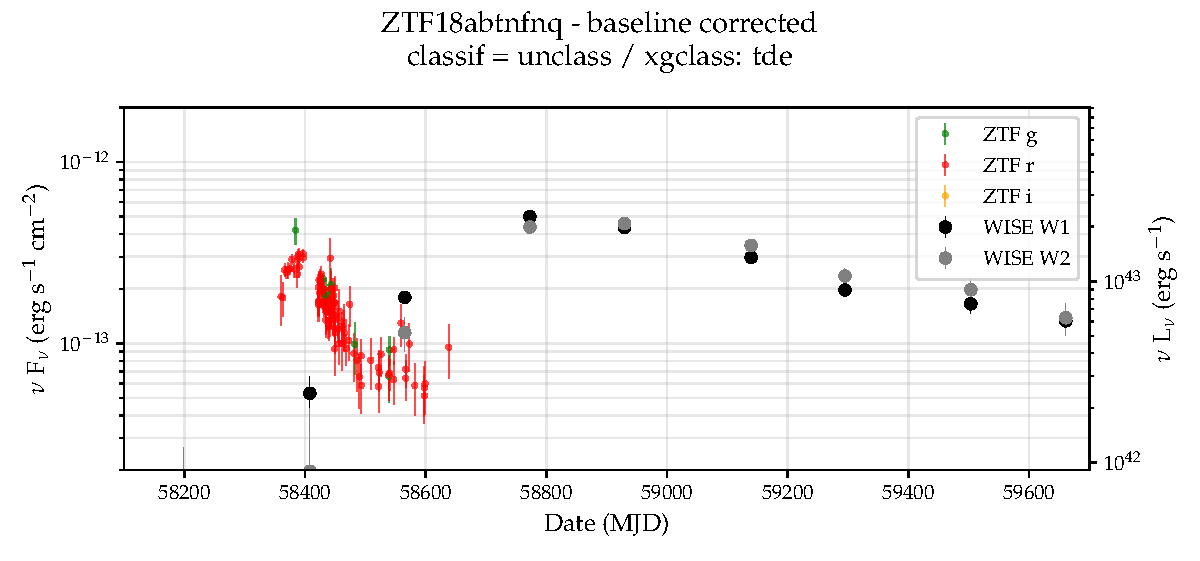
\includegraphics[width=1\textwidth]{nuclear/ZTF18abtnfnq.pdf}
  \end{subfigure}
  \begin{subfigure}[htb]{1\textwidth}
    \centering
    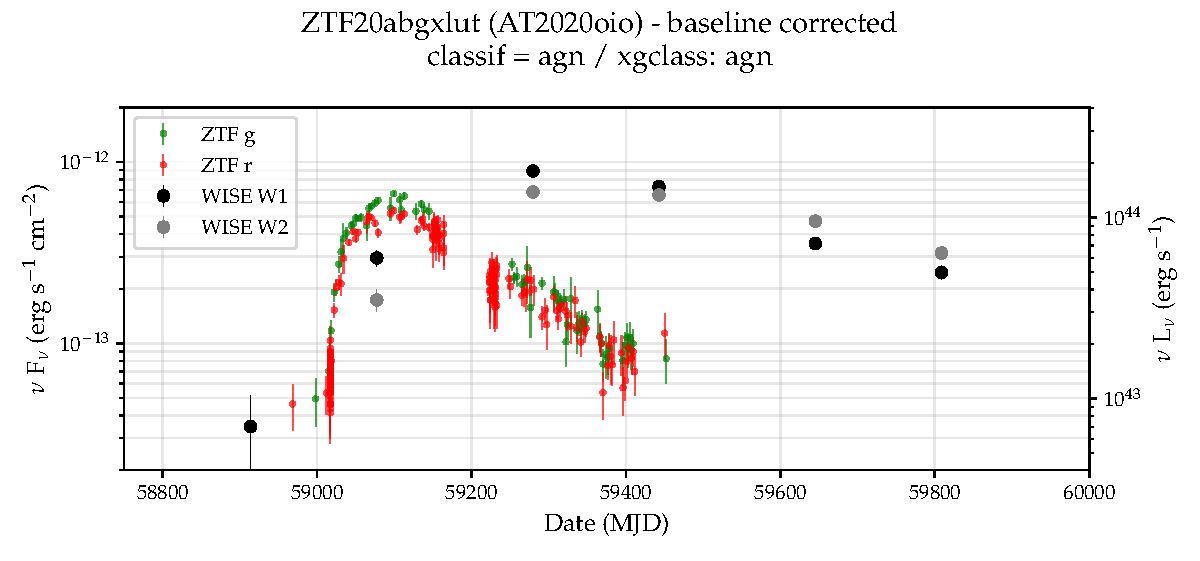
\includegraphics[width=1\textwidth]{nuclear/ZTF20abgxlut.pdf}
  \end{subfigure}
  \caption[Two exemplary light curves from the dust echo selection]{Two exemplary light curves from the dust echo section. Top: TDE candidate \textit{\href{https://ztfnuclear.simeonreusch.com/transient/ZTF18abtnfnq}{ZTF18abtnfnq}}. Bottom: Accretion flare candidate \textit{\href{https://ztfnuclear.simeonreusch.com/transient/ZTF18abtnfnq}{AT2020oio}}. Both have spectacular dust echoes. On the top, the delay between optical and infrared peak is roughly 400 days, while on the bottom it is about 180 days.}
  \labfig{two_dustecho_examples}
\end{figure}

Two exemplary light curves are shown in Fig.~\ref{fig:two_dustecho_examples}, one bona-fide candidate TDE (\textit{\href{https://ztfnuclear.simeonreusch.com/transient/ZTF18abtnfnq}{ZTF18abtnfnq}}), and one more ambiguous accretion flare similar to \textit{AT2019fdr}: \textit{\href{https://ztfnuclear.simeonreusch.com/transient/ZTF18abtnfnq}{AT2020oio}}.

One can now compare both populations, the dust-echo accompanied transients and those without. The rise and decay times resulting from the TDE fit for both can be seen in Fig.~\ref{fig:risedecay}

\begin{figure}[htb]
  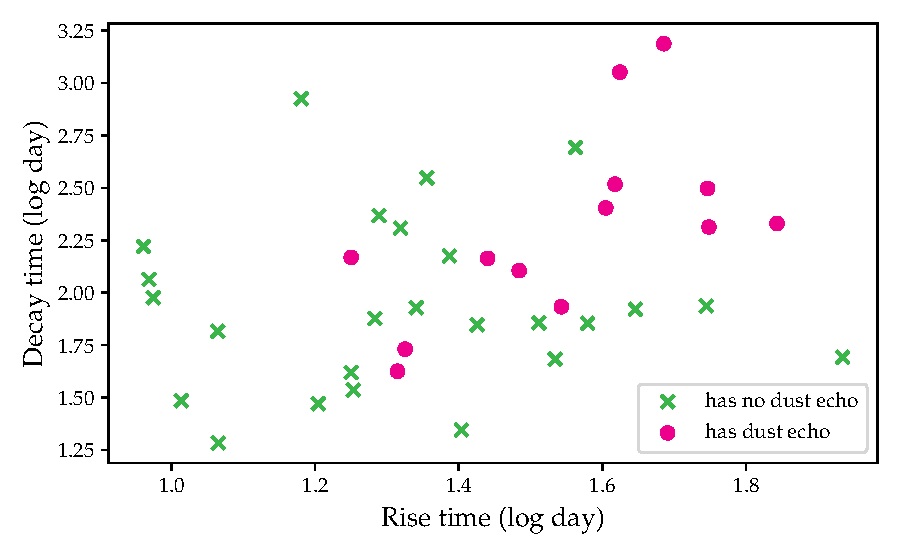
\includegraphics[width=1\textwidth]{nuclear/risedecay.pdf}
  \caption[Dust and non-dust echo rise- and decay times]{Rise and decay times for the transients accompanied by a dust echo versus those without one. Both axes are log day, and the dust-echo transients are shown as magenta dots, while the non dust-echo transients are shown as green crosses. On average, dust-echo accompanied transients evolve more slowly, suggesting a higher percentage of ambiguous nuclear transients among the dust-echo selected sample.}
  \labfig{risedecay}
\end{figure}

The two populations are by far not distinct, but a slight trend towards longer rise and decay times for the transients accompanied by a dust echo can be discerned. This suggests that the fraction of ambiguous accretion flares is higher among the dust echo sample. Partially this might be a selection effect, as the 2D cuts introduced in Section~\ref{visual_cuts} were custom-tailored to capture bona fide TDEs, while the dust-echo selection did not rely on these 2D cuts.

\subsubsection{Comparison to Flux-Complete Sample}
To check whether the number of new candidates from this work is compatible with expectations, I calculated a rough estimate on the expected number of TDEs when not limited by survey efficiency. To approximate the `true' rate of TDEs accessible by ZTF, I assumed that in the magnitude bin between 17.5 and 18.0 all TDEs were in fact discovered. With this normalization, I calculated the flux-complete numbers for each magnitude bin, assuming the TDE population follows a distribution given by $N\propto f^{-\frac{3}{2}}$, where $N$ is the expected number of TDEs and $f$ is the TDE flux.

\begin{figure}[htb]
  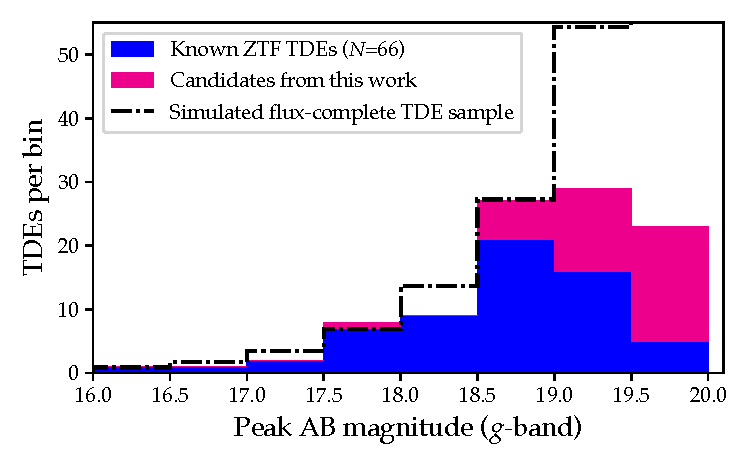
\includegraphics[width=1\textwidth]{nuclear/detection_efficiency.pdf}
  \caption[ZTF TDE detections per magnitude bin]{ZTF detected TDEs per \textit{g}-band peak magnitude bin. The 66 known TDEs are shown in blue, while all the candidates from this work are shown in magenta. Furthermore, the flux-complete TDE sample (following a $f^{-\frac{3}{2}}$ distribution), normalized to the 17.5--18 magnitude bin, is shown as black dash-dotted line.}
  \labfig{detection_efficiency}
\end{figure}

The resulting distribution is shown in Fig.~\ref{fig:detection_efficiency}, which displays the 66 known ZTF-detected TDEs used in this study (all of them fall into the time range of the nuclear sample) in blue. These are appended by the TDE candidates newly identified by this work (magenta), as well as the simulated flux-complete TDE sample (black dash-dotted line). This clearly shows that almost all candidates from this work could in fact be TDEs without violating the expected number of TDEs, especially in the two faintest magnitude bins.

This figure also highlights that even if all the TDE candidates truly were TDEs, the sample would still be far from complete at the faint end. For example, in the 19--19.5 magnitude bin, only half the number of expected TDEs is detected. This is not surprising, as the depth of ZTF survey observations does not exceed $\sim 20.5$ mag, and only transients significantly brighter at peak will display a light curve that allows for reliable photometric identification.

\section{Conclusion}\label{nuc_conclusion}
Extracting previously unknown TDE candidates from the nuclear sample by using a trained algorithm aided by 2D cuts on the one side, and vetting promising dust-echo sources on the other side yielded in total 41 new candidates. This highlights that even dedicated programs are missing some candidates. If assuming that about half of the new candidates are in fact TDEs (in contrast to AGN activity and SNe, see Section~\ref{all_tde_inspection} for a justification of that assumption), the luminosity function of TDEs might need to be adjusted. This is not exactly straightforward to do, as all the transients are over by now and the window of opportunity to classify them spectroscopically has closed. Nevertheless, the number of additional candidates and their magnitude distribution is in line with expectations when extrapolating from the ZTF-discovered TDEs in the 17.5--18.0 magnitude range.

One key takeaway from this study is that the contamination by AGN is the foremost problem in improving the quality of the photometric classifier. It seems that requiring exactly one coincident flare in two bands, and rejecting based on the reduced $\chi^2$ of the two fits does not yield enough information, leaving a set of AGN misclassified as other transients. Therefore, it would be fruitful for future studies to add another classifier designed solely to reject stochastic AGN variability by identifying periodic behavior, e.g. based on Gaussian processes.

\subsubsection{Outlook}

It might be a promising avenue to obtain the missing host redshifts for the new transients identified in this study (of the 27 \texttt{XGBoost}-classified TDE candidates, 4 have a spectroscopic redshift, 12 a photometric redshift and 11 have none). There were 16 new dust-echo accompanied candidate TDEs and accretion flares, 14 of which are not already included in the 27 \texttt{XGBoost} candidates. Of these, 6 have a spectroscopic redshift, 4 have a photometric redshift and 4 have none. One could design a small program to acquire the 31 additional spectra needed to have reliable host redshifts for all the new transients.

Such a program will have to accommodate the fact that each additional TDE candidate will be intrinsically uncertain. Nevertheless, obtaining redshifts would allow to make the TDE nature of some candidates more plausible: The possible AGN nature of host galaxies would become apparent in their spectra, and in some cases alternative SN classifications might be ruled out based on the intrinsic luminosity of the respective event.

The ZTF TDE working group has spectroscopically identified 30 TDEs within a data-taking period of 2.6 years, translating to 11.5 discoveries per year. This study identified 27 additional candidates with the \texttt{XGBoost} classifier; when assuming at least \SI{50}{\percent} of these are in fact TDEs, paired with a data-taking period of 4 years, this results in an additional 3.4 TDEs per year, an increase of \SI{29}{\percent}. Adding \SI{50}{\percent} of the candidate TDEs identified by their dust-echo results in an additional 1.75 TDEs per year.

One important remaining question concerns the differentiation between clear-cut TDEs and events which are somewhat ambiguous. The latter are in general more energetic, longer lived and occur in active galaxies. These are exemplified in Fig.~\ref{fig:two_dustecho_examples}, where \textit{ZTF18abtnfnq} is a classical TDE candidate, and \textit{ZTF20abgxlut} is more luminous, longer lived and situated in an AGN. One could hypothesize that both populations do in fact form a continuum; the classical TDEs on one end, and tidal disruptions happening in the environments of active galaxies on the other end, together constituting the class of `accretion flares'.

Consequently, timely acquisition of spectroscopy is crucial in studying this possible continuum further; and the real-time application of the classifier developed in this work might be a promising avenue. Of course, such an application will have to deal with much younger and therefore shorter light curves and the fact that the transients are still evolving. Nevertheless, this can be done, as~\sidecite{Miranda2022} have shown for the more general case of identifying transients worthy of early spectroscopic follow-up. Several of the features used by the classifier in this work will pose no problem, but the fit-based ones will need adjustments to allow the fitting of transients which are either young, or at least still evolving.

Additionally, along the lines of~\cite{Velzen2021}, this study gave further evidence that the existence of a strong infrared flare is a good predictor for TDE-like behavior. We have successfully used an algorithm identifying periods of flaring activity which are then automatically checked if they could constitute a dust echo. Systematically using \textit{WISE} data releases as soon as they are published to power an automatic pipeline searching for promising transients accompanied by dust echoes seems to be a promising avenue of research. This would also increase the fraction of spectroscopically classified transients belonging to the ambiguous `accretion flare' category, possibly shedding more light on their nature.

It remains to be seen if dust-echo accompanied TDEs are in fact emitters of high-energy neutrinos. This work on \textit{AT2019fdr} and the study additionally highlighting \textit{AT2019aalc}~\cite{Velzen2021} found evidence in favor of that hypothesis. On the other hand, when crossmatching the transients of that study with the full catalog of IceCube alerts---not only the alert neutrinos---\sidecite{Necker2023b} found no significant correlation. If the neutrino spectrum is hard enough, these two results do not contradict each other, though. Crossmatching the increased sample of dust-echo accompanied TDE candidates created in this work will shed more light on that question: The sample created here has a higher quality than what was used in~\cite{Velzen2021}, as the time range of observations is longer and there was a visual selection of TDE-like transients, rendering the sample more pure.


% fehler in der diskussion des beispielfits von AT2019dsg einbauen

% normierung purity im finalen resultat
% die ausgezeichnete 

% confusion matrices vielleicht mit produkt, bisschen zusammenkürzen? produkt aus beidem
% mit frequenz wie oft sowas tatsächclich vorkommt

% - sensitivität und spezifität / tatsächliche verteilung ableiten von BTS



% The 24 objects classified as TDEs that were lying in AGN hosts were also evaluated. Unfortunately, visual inspection of these events ruled out all but one (\textit{ZTF18acryjql}) transient.  -> BEISPIEL; VISUALISIEREN
% zero-prävalenz


% 50% purity, bisschen diskutieren, wo man dann steht. Würde man das erwarten? Bisschen extrapolieren von dem, was man im BTS schon sieht.

% In den conclusions vom nuclear sample bisschen weniger zukunft, sondern erklären, warum was nötig wäre.
% AGN rejection nicht gut genug DAS IST DIE ERKLÄRUNG

